% 原书第3--8页至题型一结束；PDF第11--16页。人工对照原页转写。
\chapter{矩阵与线性变换}
高等代数内容包括：线性代数和多项式。本章重点关注矩阵与线性变换。
由于线性变换可用矩阵表示，本质上讲研究线性变换也就是研究矩阵。
因此我们讨论的主要内容包括矩阵的运算、线性变换的基本性质，以及矩阵的行列式、矩阵的特征值和特征向量、矩阵的秩、矩阵的迹等。
这些是线性代数的基础部分，特别地，矩阵与行列式是两个最基本的概念，熟练掌握它们的性质是最基本的要求。

\section{竞赛要点与难点}
\begin{enumerate}[label=（\arabic*）]
\item 矩阵的概念，矩阵的运算（加法、数乘、乘法、转置等运算）及其运算律。
\item 矩阵乘积的行列式、矩阵乘积的秩与其因子的秩的关系。
\item 矩阵的逆、伴随矩阵、矩阵可逆的条件，初等矩阵、初等变换、矩阵的等价标准形及逆矩阵的求解等。
\item 分块矩阵：分块矩阵及其运算与性质，分块初等矩阵、分块初等变换及其应用等。
\item 行列式的定义：2阶、3阶行列式的定义及对角线法则，排列与逆序数，$n$级行列式的定义等。
\item 行列式的性质。
\item 行列式的计算：根据定义计算行列式，利用行列式性质计算行列式，行列式行（列）展开、Laplace（拉普拉斯）展开定理等。
\item Cramer（克拉默）法则。
\item 矩阵的行秩、列秩、秩、矩阵的秩与其子式的关系。
\item 线性变换的定义、线性变换的运算、线性变换的矩阵。
\item 特征值与特征向量：线性变换和矩阵的特征值与特征向量、可对角化线性变换和矩阵的性质与判定、相似矩阵、相似不变量、Hamilton--Cayley（哈密顿--凯莱）定理等。
\item $\lambda$-矩阵：$\lambda$-矩阵、$\lambda$-矩阵在初等变换下的标准形、行列式因子、不变因子、初等因子，矩阵相似的条件等。
\item Jordan（若尔当）矩阵、Jordan标准形、有理标准形。
\end{enumerate}

\section{范例解析与精讲}
\subsection*{题型一\quad 矩阵的运算}
矩阵的运算中需要注意矩阵乘法不满足交换律，同时矩阵中有零因子存在，即两个非零矩阵乘积可以等于零矩阵。概括起来，以下几点需要特别注意：
\begin{enumerate}[label=（\arabic*）]
\item 一般地，二项式定理
\[
(A+B)^n=\sum_{i=0}^n\binom ni A^iB^{n-i}
\]
不一定成立。但若$A,B$可交换，即$AB=BA$，则上式成立。
\item 矩阵乘法没有消去律，即$CX=CY$（或$XC=YC$）推不出$X=Y$。但是有如下特别结论：
\begin{enumerate}[label=（\roman*）]
\item 一个矩阵$C$左可消当且仅当$C$为列满秩，即以下两条陈述等价：
\begin{enumerate}[label=（\alph*）]
\item 由$CX=CY$可推出$X=Y$。
\item $C$是列满秩，即$C$的列向量组线性无关或者$\rank(C)=C$的列数。
\end{enumerate}
\item 一个矩阵$C$右可消当且仅当$C$为行满秩，即以下两条陈述等价：
\begin{enumerate}[label=（\alph*）]
\item 由$XC=YC$可推出$X=Y$。
\item $C$是行满秩，即$C$的行向量组线性无关或者$\rank(C)=C$的行数。
\end{enumerate}
\item $A^2=E$推不出$A=E$或$A=-E$，即$A^2-E=(A+E)(A-E)=O$推不出$A+E=O$或$A-E=O$。
\end{enumerate}
\end{enumerate}

\ex{1.2.1}设$A,B$均是$n$阶方阵且满足$A^2=A$，$B^2=B$，$(A+B)^2=A+B$，求$AB$。
\sol 由$(A+B)^2=A+B$得到
\[A^2+AB+BA+B^2=A+B.\]
又$A^2=A$，$B^2=B$，所以
\[AB=-BA,\]
从而
\[A\cdot AB=-A\cdot BA,\]
即
\[AB=-ABA;\]
\[AB\cdot A=-BA\cdot A,\]
即
\[ABA=-BA\quad\text{或}\quad BA=-ABA,\]
因此
\[AB=BA.\]
由此得到$2AB=O$，故有$AB=O$。

\ex{1.2.3}设
\[
A=\begin{pmatrix}
a_1b_1&a_1b_2&\cdots&a_1b_n\\
a_2b_1&a_2b_2&\cdots&a_2b_n\\
\vdots&\vdots&&\vdots\\
a_nb_1&a_nb_2&\cdots&a_nb_n
\end{pmatrix},
\]
$k$为正整数，求$A^k$。
\sol $A$可分解为
\[
A=\begin{pmatrix}a_1\\a_2\\\vdots\\a_n\end{pmatrix}
\begin{pmatrix}b_1&b_2&\cdots&b_n\end{pmatrix}
=\alpha\beta^{\mathrm T},
\]
其中
\[
\alpha=\begin{pmatrix}a_1\\a_2\\\vdots\\a_n\end{pmatrix},\qquad
\beta=\begin{pmatrix}b_1\\b_2\\\vdots\\b_n\end{pmatrix},
\]
所以
\begin{align*}
A^k&=\underbrace{(\alpha\beta^{\mathrm T})(\alpha\beta^{\mathrm T})\cdots(\alpha\beta^{\mathrm T})}_{k\text{个}}\\
&=\alpha\underbrace{(\beta^{\mathrm T}\alpha)(\beta^{\mathrm T}\alpha)\cdots(\beta^{\mathrm T}\alpha)}_{k-1\text{个}}\beta^{\mathrm T}\\
&=\alpha(\beta^{\mathrm T}\alpha)^{k-1}\beta^{\mathrm T},
\end{align*}
而
\[\beta^{\mathrm T}\alpha=a_1b_1+a_2b_2+\cdots+a_nb_n,\]
故有
\begin{align*}
A^k&=(a_1b_1+a_2b_2+\cdots+a_nb_n)^{k-1}A\\
&=(a_1b_1+a_2b_2+\cdots+a_nb_n)^{k-1}
\begin{pmatrix}
a_1b_1&a_1b_2&\cdots&a_1b_n\\
a_2b_1&a_2b_2&\cdots&a_2b_n\\
\vdots&\vdots&&\vdots\\
a_nb_1&a_nb_2&\cdots&a_nb_n
\end{pmatrix}.
\end{align*}

\ex{1.2.5}设
\[
A=\begin{pmatrix}
2&0&0&0&0&0\\
3&2&0&0&0&0\\
0&3&2&0&0&0\\
0&0&0&1&2&0\\
0&0&0&0&1&2\\
0&0&0&0&0&1
\end{pmatrix},
\]
求$A^{100}$。
\sol 设
\[
A_1=\begin{pmatrix}2&0&0\\3&2&0\\0&3&2\end{pmatrix},\qquad
A_2=\begin{pmatrix}1&2&0\\0&1&2\\0&0&1\end{pmatrix}.
\]
则$A$可写为如下分块形式：
\[A=\begin{pmatrix}A_1&\\&A_2\end{pmatrix},\]
于是
\[A^{100}=\begin{pmatrix}A_1^{100}&\\&A_2^{100}\end{pmatrix}.\]
将$A_1,A_2$分解为
\[
A_1=2E+3S,\qquad\text{其中}\quad
S=\begin{pmatrix}0&0&0\\1&0&0\\0&1&0\end{pmatrix};
\]
\[
A_2=E+2H,\qquad\text{其中}\quad
H=\begin{pmatrix}0&1&0\\0&0&1\\0&0&0\end{pmatrix}.
\]
注意到$S$与$E$、$H$与$E$均可交换且
\[
S^2=\begin{pmatrix}0&0&0\\0&0&0\\1&0&0\end{pmatrix},\qquad
S^i=O\quad(i\ge3),
\]
\[
H^2=\begin{pmatrix}0&0&1\\0&0&0\\0&0&0\end{pmatrix},\qquad
H^i=O\quad(i\ge3).
\]
由二项式定理
\begin{align*}
A_1^{100}
&=(2E+3S)^{100}=\sum_{i=0}^{100}\binom{100}{i}(2E)^{100-i}(3S)^i\\
&=\binom{100}{0}(2E)^{100}
 +\binom{100}{1}(2E)^{99}\cdot3S
 +\binom{100}{2}(2E)^{98}(3S)^2\\
&=2^{100}E+300S\cdot2^{99}E
 +\frac{100\times99}{2}\cdot9S^2\cdot2^{98}E\\
&=2^{100}E+300\cdot2^{99}\cdot S+50\cdot99\cdot9\cdot2^{98}\cdot S^2\\
&=\begin{pmatrix}
2^{100}&0&0\\
3\cdot5^2\cdot2^{101}&2^{100}&0\\
11\cdot5^2\cdot3^4\cdot2^{99}&3\cdot5^2\cdot2^{101}&2^{100}
\end{pmatrix},
\end{align*}
\begin{align*}
A_2^{100}
&=(E+2H)^{100}
 =E^{100}+100\cdot E^{99}\cdot(2H)
 +\frac{100\times99}{2}\cdot E^{98}\cdot(2H)^2\\
&=E+200H+19800H^2\\
&=\begin{pmatrix}1&200&19800\\0&1&200\\0&0&1\end{pmatrix}.
\end{align*}
因此
\[
\setlength{\arraycolsep}{3pt}
A^{100}=\begin{pmatrix}
2^{100}&0&0&0&0&0\\
3\cdot5^2\cdot2^{101}&2^{100}&0&0&0&0\\
11\cdot5^2\cdot3^4\cdot2^{99}&3\cdot5^2\cdot2^{101}&2^{100}&0&0&0\\
0&0&0&1&200&19800\\
0&0&0&0&1&200\\
0&0&0&0&0&1
\end{pmatrix}.
\]

\par\medskip\noindent\textbf{总结}\quad 计算方阵的方幂一般有三种方法：
\begin{enumerate}[label=（\arabic*）]
\item 基于相似变换的计算法。更常见的情形是利用相似标准形（比如Jordan标准形）来进行计算。
\item 利用递推公式法或者说数学归纳法，如例1.2.3。
\item 基于方阵分解，然后利用二项式定理来进行计算，如例1.2.5。
\end{enumerate}

\subsection*{题型二\quad 矩阵可逆的判定及计算}

% SOURCE_PDF_PAGE 16

\hypertarget{source-p016}{}
\sourceblock{171.76}{images-full/p016-d000.png}
命题设$A$ 为$n$ 阶矩阵则有
\sourceblock{238.99}{images-full/p016-d001.png}


% SOURCE_PDF_PAGE 17

\hypertarget{source-p017}{}
\allowbreak{}\raisebox{-2.40pt}{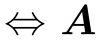
\includegraphics[width=28.81pt]{images-full/p017-i000.png}}\allowbreak{} 的特征值均不为0
\allowbreak{}\raisebox{-2.28pt}{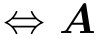
\includegraphics[width=28.25pt]{images-full/p017-i001.png}}\allowbreak{} 的伴随矩阵\allowbreak{}\raisebox{-2.40pt}{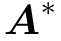
\includegraphics[width=16.95pt]{images-full/p017-i002.png}}\allowbreak{} 可逆
\allowbreak{}\raisebox{-2.28pt}{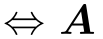
\includegraphics[width=28.81pt]{images-full/p017-i003.png}}\allowbreak{} 是一些初等矩阵之积.
\par\medskip\noindent\textbf{【例1.2.6 】设\allowbreak{}\raisebox{-2.76pt}{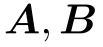
\includegraphics[width=28.81pt]{images-full/p017-i004.png}}\allowbreak{} 均为$n$ 阶方阵若\allowbreak{}\raisebox{-2.28pt}{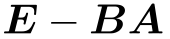
\includegraphics[width=47.77pt]{images-full/p017-i006.png}}\allowbreak{} 可逆，证明\allowbreak{}\raisebox{-2.28pt}{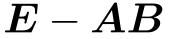
\includegraphics[width=47.93pt]{images-full/p017-i007.png}}\allowbreak{} 可逆，并求}
\sourceblock{355.38}{images-full/p017-d000.png}
因此
\sourceblock{192.66}{images-full/p017-d001.png}
由于\allowbreak{}\raisebox{-2.28pt}{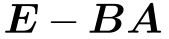
\includegraphics[width=47.46pt]{images-full/p017-i008.png}}\allowbreak{} 可逆，即\allowbreak{}\raisebox{-3.00pt}{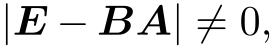
\includegraphics[width=77.97pt]{images-full/p017-i009.png}}\allowbreak{}，所以\allowbreak{}\raisebox{-3.00pt}{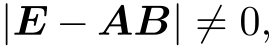
\includegraphics[width=75.78pt]{images-full/p017-i010.png}}\allowbreak{}，因此\allowbreak{}\raisebox{-2.28pt}{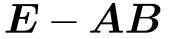
\includegraphics[width=47.36pt]{images-full/p017-i011.png}}\allowbreak{} 可逆. 下
面进一步求\allowbreak{}\raisebox{-3.24pt}{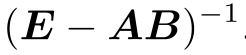
\includegraphics[width=69.39pt]{images-full/p017-i012.png}}\allowbreak{} 由于
\sourceblock{185.88}{images-full/p017-d002.png}
故
\sourceblock{228.26}{images-full/p017-d003.png}
进而
\sourceblock{201.14}{images-full/p017-d004.png}
\sourceblock{326.57}{images-full/p019-d002.png}
\sourceblock{276.85}{images-full/p019-d003.png}
\par\noindent (3) 定义法，由\allowbreak{}\raisebox{-2.28pt}{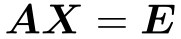
\includegraphics[width=50.85pt]{images-full/p019-i004.png}}\allowbreak{} 求出\allowbreak{}\raisebox{-2.28pt}{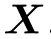
\includegraphics[width=14.16pt]{images-full/p019-i005.png}}\allowbreak{}
若矩阵$A$ 没有具体给出，是抽象的，则首先想到的是用定义来求\allowbreak{}\raisebox{-2.76pt}{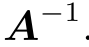
\includegraphics[width=24.62pt]{images-full/p019-i007.png}}\allowbreak{}.
\sourceblock{300.01}{images-full/p022-d004.png}
矩阵的行列式是矩阵的一个数值特征.矩阵的数值特征还有矩阵的秩、矩阵的特征
\sourceblock{357.64}{images-full/p022-d005.png}
\sourceblock{132.21}{images-full/p022-d006.png}
计算\allowbreak{}\raisebox{-3.00pt}{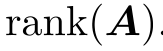
\includegraphics[width=45.83pt]{images-full/p022-i000.png}}\allowbreak{}


% SOURCE_PDF_PAGE 23

\hypertarget{source-p023}{}
\par\noindent\textbf{解}\ 
\sourceblock{389.85}{images-full/p023-d000.png}
\sourceblock{450.00}{images-full/p023-d001.png}
\par\medskip\noindent\textbf{【例1.2.13 】设$A$ 为2023 阶非军实矩阵. \allowbreak{}\raisebox{-3.00pt}{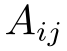
\includegraphics[width=18.64pt]{images-full/p023-i001.png}}\allowbreak{} 为$A$ 中元素\allowbreak{}\raisebox{-2.28pt}{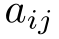
\includegraphics[width=16.38pt]{images-full/p023-i003.png}}\allowbreak{}的代数余子式且}
\allowbreak{}\raisebox{-3.00pt}{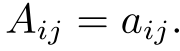
\includegraphics[width=50.51pt]{images-full/p023-i004.png}}\allowbreak{}·求$A$ 的秩与行列式.
解由于\allowbreak{}\raisebox{-2.76pt}{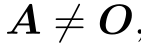
\includegraphics[width=39.55pt]{images-full/p023-i006.png}}\allowbreak{}，不妨设\allowbreak{}\raisebox{-2.76pt}{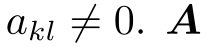
\includegraphics[width=58.17pt]{images-full/p023-i007.png}}\allowbreak{} 按第$k$ 行展开有
\sourceblock{166.67}{images-full/p023-d002.png}
故\allowbreak{}\raisebox{-3.00pt}{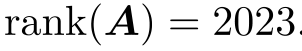
\includegraphics[width=84.87pt]{images-full/p023-i009.png}}\allowbreak{}.
由己知布$A$ 的伴随矩阵\allowbreak{}\raisebox{-2.76pt}{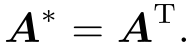
\includegraphics[width=52.75pt]{images-full/p023-i011.png}}\allowbreak{}所以由\allowbreak{}\raisebox{-3.00pt}{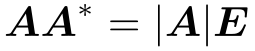
\includegraphics[width=71.75pt]{images-full/p023-i012.png}}\allowbreak{} 有\allowbreak{}\raisebox{-3.36pt}{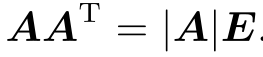
\includegraphics[width=74.22pt]{images-full/p023-i013.png}}\allowbreak{}. 两边取
行列式有
\sourceblock{328.26}{images-full/p023-d003.png}
\sourceblock{416.97}{images-full/p024-d001.png}
解根据rank(A) 的情况讨论
\sourceblock{450.00}{images-full/p024-d002.png}
\sourceblock{450.00}{images-full/p024-d003.png}
\sourceblock{344.65}{images-full/p024-d004.png}


% SOURCE_PDF_PAGE 25

\hypertarget{source-p025}{}
设矩阵$A$ 的特征值为\allowbreak{}\raisebox{-2.76pt}{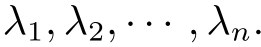
\includegraphics[width=73.36pt]{images-full/p025-i001.png}}\allowbreak{} 求矩阵$B$ 的特征值.
解矩阵$A$ 和$B$ 的特征多项式分别为
\sourceblock{272.33}{images-full/p025-d000.png}
\sourceblock{311.88}{images-full/p025-d001.png}
当$n=l$ 时，
\sourceblock{140.12}{images-full/p025-d002.png}
当\allowbreak{}\raisebox{-2.28pt}{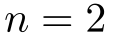
\includegraphics[width=31.64pt]{images-full/p025-i006.png}}\allowbreak{} 时，
\sourceblock{287.02}{images-full/p025-d003.png}
\sourceblock{107.35}{images-full/p025-d004.png}
设\allowbreak{}\raisebox{-2.64pt}{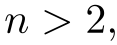
\includegraphics[width=32.85pt]{images-full/p025-i007.png}}\allowbreak{}则有
\sourceblock{256.51}{images-full/p025-d005.png}
\sourceblock{450.00}{images-full/p025-d006.png}
\par\medskip\noindent\textbf{【例1.2.17】设1013 阶实方阵$A$ 可对角化且满足}
\sourceblock{141.25}{images-full/p025-d007.png}


% SOURCE_PDF_PAGE 26

\hypertarget{source-p026}{}
和
\sourceblock{101.13}{images-full/p026-d000.png}
求$A$ 的特征值.
解由于$A$ 可对角化，故$A$ 的每个特征值的代数重数等于其几何重数.令\allowbreak{}\raisebox{-2.28pt}{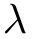
\includegraphics[width=9.04pt]{images-full/p026-i003.png}}\allowbreak{} 为$A$
的特征值，则有
\sourceblock{122.04}{images-full/p026-d001.png}
即
\sourceblock{117.52}{images-full/p026-d002.png}
\sourceblock{107.35}{images-full/p026-d003.png}
故$A$ 的特征值只可能是\allowbreak{}\raisebox{-2.64pt}{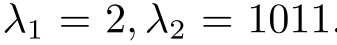
\includegraphics[width=94.83pt]{images-full/p026-i006.png}}\allowbreak{}.注意到\allowbreak{}\raisebox{-3.00pt}{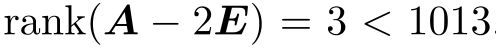
\includegraphics[width=139.88pt]{images-full/p026-i007.png}}\allowbreak{} 所以2
是$A$ 的一个特征值.
由于可对角化，特征值2 的代数重数等于其几何重数.由于\allowbreak{}\raisebox{-3.00pt}{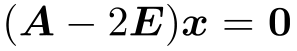
\includegraphics[width=83.62pt]{images-full/p026-i009.png}}\allowbreak{} 的解空
间维数为\allowbreak{}\raisebox{-3.00pt}{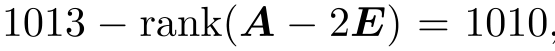
\includegraphics[width=156.52pt]{images-full/p026-i010.png}}\allowbreak{}，因此2 作为$A$ 的特征值，其代数重数为1010.
故$A$ 还有其他特征值，且一定为1011. 其代数重数为\allowbreak{}\raisebox{-2.16pt}{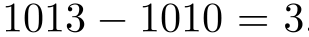
\includegraphics[width=86.91pt]{images-full/p026-i013.png}}\allowbreak{} 至此$A$ 的全部
特征值为\allowbreak{}\raisebox{-3.00pt}{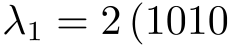
\includegraphics[width=66.10pt]{images-full/p026-i015.png}}\allowbreak{} 重)，\allowbreak{}\raisebox{-3.00pt}{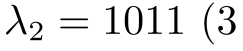
\includegraphics[width=68.36pt]{images-full/p026-i016.png}}\allowbreak{} 重) .
【注1.2.31前面例1.2.16 和例1.2.17 考察的是抽象矩阵特征值的计算问题.
\par\medskip\noindent\textbf{【例1.2.18 】设$A$ 为3 阶实对称矩阵，\allowbreak{}\raisebox{-3.00pt}{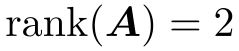
\includegraphics[width=67.23pt]{images-full/p026-i018.png}}\allowbreak{} 且}
\sourceblock{285.32}{images-full/p026-d004.png}
\par\noindent (2) 矩阵$A$
\sourceblock{450.00}{images-full/p026-d005.png}
属于特征值。的特征向量，则有


% SOURCE_PDF_PAGE 27

\hypertarget{source-p027}{}
\sourceblock{79.10}{images-full/p027-d000.png}
\sourceblock{346.91}{images-full/p027-d001.png}
\sourceblock{375.16}{images-full/p027-d002.png}
\sourceblock{410.19}{images-full/p027-d003.png}
的全部特征值.
解(方法1) 首先计算\allowbreak{}\raisebox{-2.88pt}{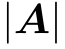
\includegraphics[width=18.08pt]{images-full/p027-i000.png}}\allowbreak{} 以便确定。是否为$A$ 的特征值.易知


% SOURCE_PDF_PAGE 28

\hypertarget{source-p028}{}
\sourceblock{240.12}{images-full/p028-d000.png}
故\allowbreak{}\raisebox{-2.28pt}{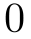
\includegraphics[width=8.47pt]{images-full/p028-i000.png}}\allowbreak{} 是$A$ 的特征值.下面确定\allowbreak{}\raisebox{-2.28pt}{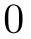
\includegraphics[width=8.47pt]{images-full/p028-i002.png}}\allowbreak{} 的代数重数.
由于\allowbreak{}\raisebox{-3.00pt}{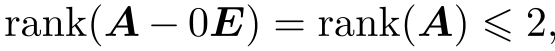
\includegraphics[width=156.43pt]{images-full/p028-i003.png}}\allowbreak{}，因此\allowbreak{}\raisebox{-2.28pt}{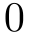
\includegraphics[width=8.47pt]{images-full/p028-i004.png}}\allowbreak{} 的代数重数\allowbreak{}\raisebox{-2.52pt}{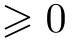
\includegraphics[width=20.34pt]{images-full/p028-i005.png}}\allowbreak{} 的儿何重数\allowbreak{}\raisebox{-2.64pt}{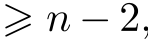
\includegraphics[width=41.44pt]{images-full/p028-i006.png}}\allowbreak{}，即
$A$ 至少有\allowbreak{}\raisebox{-2.16pt}{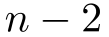
\includegraphics[width=30.51pt]{images-full/p028-i008.png}}\allowbreak{} 个特征值为\allowbreak{}\raisebox{-2.16pt}{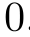
\includegraphics[width=8.12pt]{images-full/p028-i009.png}}\allowbreak{}
\sourceblock{205.09}{images-full/p028-d001.png}
\sourceblock{390.98}{images-full/p028-d002.png}
故\allowbreak{}\raisebox{-2.28pt}{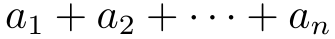
\includegraphics[width=94.35pt]{images-full/p028-i010.png}}\allowbreak{}也是$A$ 的特征值，而
\sourceblock{226.56}{images-full/p028-d003.png}
故\allowbreak{}\raisebox{-2.64pt}{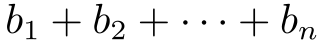
\includegraphics[width=90.96pt]{images-full/p028-i012.png}}\allowbreak{} 是\allowbreak{}\raisebox{-2.76pt}{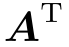
\includegraphics[width=19.21pt]{images-full/p028-i013.png}}\allowbreak{} 的特征值.从丽也是$A$ 的特征值.
\sourceblock{372.33}{images-full/p028-d004.png}
若\allowbreak{}\raisebox{-2.88pt}{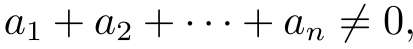
\includegraphics[width=116.29pt]{images-full/p028-i015.png}}\allowbreak{}，则\allowbreak{}\raisebox{-2.40pt}{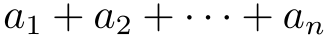
\includegraphics[width=93.22pt]{images-full/p028-i016.png}}\allowbreak{}为$A$ 的一个非零特征值，从而\allowbreak{}\raisebox{-2.64pt}{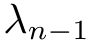
\includegraphics[width=25.99pt]{images-full/p028-i018.png}}\allowbreak{}
\sourceblock{450.00}{images-full/p028-d005.png}
最后考察\allowbreak{}\raisebox{-2.64pt}{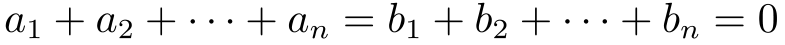
\includegraphics[width=221.48pt]{images-full/p028-i019.png}}\allowbreak{} 的情形.
注意到$A$ 的特征多项式\allowbreak{}\raisebox{-2.76pt}{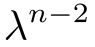
\includegraphics[width=26.55pt]{images-full/p028-i021.png}}\allowbreak{} 的系数是$A$ 的所有三阶主子式之和. 从而
\sourceblock{194.92}{images-full/p028-d006.png}


% SOURCE_PDF_PAGE 29

\hypertarget{source-p029}{}
\sourceblock{236.17}{images-full/p029-d000.png}
\sourceblock{351.99}{images-full/p029-d001.png}
因此\allowbreak{}\raisebox{-2.76pt}{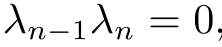
\includegraphics[width=62.41pt]{images-full/p029-i000.png}}\allowbreak{}，又\allowbreak{}\raisebox{-2.76pt}{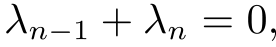
\includegraphics[width=77.76pt]{images-full/p029-i001.png}}\allowbreak{}，从而\allowbreak{}\raisebox{-2.64pt}{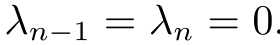
\includegraphics[width=78.78pt]{images-full/p029-i002.png}}\allowbreak{} 这时$A$ 的全部特征值均
为\allowbreak{}\raisebox{-3.00pt}{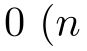
\includegraphics[width=24.29pt]{images-full/p029-i004.png}}\allowbreak{} 重).
(方法2) 根据题设可知，矩阵$A$ 可表示为
\sourceblock{241.82}{images-full/p029-d002.png}
其中
\sourceblock{248.03}{images-full/p029-d003.png}
利用行列式降阶公式，矩阵$A$ 的特征多项式可化为
\sourceblock{232.21}{images-full/p029-d004.png}
\sourceblock{274.02}{images-full/p029-d005.png}


% SOURCE_PDF_PAGE 30

\hypertarget{source-p030}{}
\sourceblock{367.81}{images-full/p030-d000.png}
\sourceblock{416.40}{images-full/p030-d001.png}
\sourceblock{330.52}{images-full/p030-d002.png}
\sourceblock{157.63}{images-full/p030-d003.png}
\sourceblock{106.78}{images-full/p030-d004.png}
\sourceblock{92.09}{images-full/p030-d005.png}
以及tr(A) 为A 的n 个特征值的和.
\sourceblock{248.03}{images-full/p030-d006.png}
解容易计算
\sourceblock{233.34}{images-full/p030-d007.png}
利用数学归纳法容易证明
\sourceblock{238.99}{images-full/p030-d008.png}
从而
\sourceblock{177.97}{images-full/p030-d009.png}


% SOURCE_PDF_PAGE 31

\hypertarget{source-p031}{}
\sourceblock{450.00}{images-full/p031-d000.png}
\sourceblock{450.00}{images-full/p031-d001.png}
矩阵，所以\allowbreak{}\raisebox{-2.52pt}{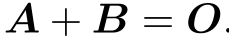
\includegraphics[width=64.40pt]{images-full/p031-i000.png}}\allowbreak{}
\sourceblock{433.35}{images-full/p031-d002.png}
$A$ 为对称矩阵
\par\noindent\textbf{证明}\ 由于
\sourceblock{163.85}{images-full/p031-d003.png}
所以
\sourceblock{355.38}{images-full/p031-d004.png}
即$A$ 为对称矩阵.口


% SOURCE_PDF_PAGE 32

\hypertarget{source-p032}{}
园也型A据眸圳特征份估针咱也
线性代数中常考虑、关于矩阵特征值、秩、迹等数值特征的估计问题.这类问题多以不
等式形式出现.解决此类问题时大多需利用相关的性质.有时还需要较强的技巧.
\sourceblock{450.00}{images-full/p032-d007.png}


% SOURCE_PDF_PAGE 33

\hypertarget{source-p033}{}
\par\noindent\textbf{证明}\ 若\allowbreak{}\raisebox{-2.76pt}{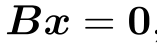
\includegraphics[width=44.21pt]{images-full/p033-i000.png}}\allowbreak{}，则\allowbreak{}\raisebox{-2.76pt}{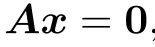
\includegraphics[width=43.37pt]{images-full/p033-i001.png}}\allowbreak{}，因而\allowbreak{}\raisebox{-3.00pt}{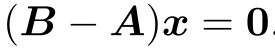
\includegraphics[width=77.37pt]{images-full/p033-i002.png}}\allowbreak{} 故\allowbreak{}\raisebox{-3.00pt}{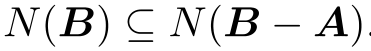
\includegraphics[width=104.59pt]{images-full/p033-i003.png}}\allowbreak{} 因此
\sourceblock{287.58}{images-full/p033-d000.png}
从而
\sourceblock{289.84}{images-full/p033-d001.png}
\sourceblock{401.15}{images-full/p033-d002.png}
\sourceblock{450.00}{images-full/p033-d003.png}
取$B$ 为单位矩阵，即得Sylvester 不等式.
\par\medskip\noindent\textbf{【例1.2.25 】设\allowbreak{}\raisebox{-2.76pt}{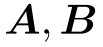
\includegraphics[width=28.81pt]{images-full/p033-i005.png}}\allowbreak{} 为$n$ 阶矩阵，\allowbreak{}\raisebox{-2.40pt}{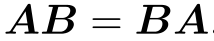
\includegraphics[width=60.29pt]{images-full/p033-i007.png}}\allowbreak{} 证明}
\sourceblock{259.33}{images-full/p033-d004.png}
\par\noindent\textbf{证明}\ 由\allowbreak{}\raisebox{-2.40pt}{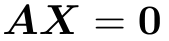
\includegraphics[width=47.46pt]{images-full/p033-i008.png}}\allowbreak{} 和\allowbreak{}\raisebox{-2.28pt}{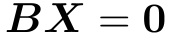
\includegraphics[width=48.02pt]{images-full/p033-i009.png}}\allowbreak{} 有\allowbreak{}\raisebox{-3.00pt}{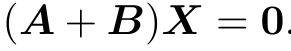
\includegraphics[width=81.84pt]{images-full/p033-i010.png}}\allowbreak{} 从而
\sourceblock{150.85}{images-full/p033-d005.png}
显然
\sourceblock{407.93}{images-full/p033-d006.png}
\sourceblock{370.07}{images-full/p033-d007.png}
故\allowbreak{}\raisebox{-3.00pt}{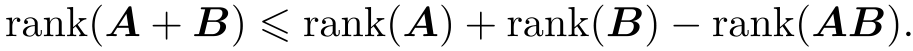
\includegraphics[width=257.70pt]{images-full/p033-i011.png}}\allowbreak{} 口


% SOURCE_PDF_PAGE 34

\hypertarget{source-p034}{}
\sourceblock{450.00}{images-full/p034-d000.png}
\sourceblock{332.22}{images-full/p034-d001.png}
可得
\sourceblock{296.06}{images-full/p034-d002.png}
\par\medskip\noindent\textbf{【例1.2.27】设$A$ 为$n$ 阶反对称实矩阵.证明关于$X$ 的矩阵方程\allowbreak{}\raisebox{-2.40pt}{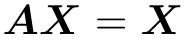
\includegraphics[width=53.11pt]{images-full/p034-i003.png}}\allowbreak{} 只}
有零解.
\par\noindent\textbf{证明}\ 由\allowbreak{}\raisebox{-2.28pt}{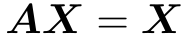
\includegraphics[width=52.54pt]{images-full/p034-i004.png}}\allowbreak{} 得\allowbreak{}\raisebox{-3.24pt}{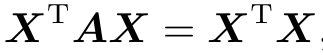
\includegraphics[width=90.88pt]{images-full/p034-i005.png}}\allowbreak{}，于是
\sourceblock{312.44}{images-full/p034-d003.png}
从而\allowbreak{}\raisebox{-3.48pt}{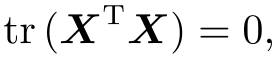
\includegraphics[width=78.43pt]{images-full/p034-i006.png}}\allowbreak{}，所以\allowbreak{}\raisebox{-2.28pt}{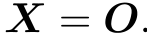
\includegraphics[width=41.22pt]{images-full/p034-i007.png}}\allowbreak{}口
\sourceblock{372.33}{images-full/p034-d004.png}
\par\noindent\textbf{证明}\ 令\allowbreak{}\raisebox{-3.00pt}{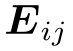
\includegraphics[width=20.34pt]{images-full/p034-i008.png}}\allowbreak{}表示\allowbreak{}\raisebox{-3.00pt}{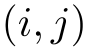
\includegraphics[width=25.42pt]{images-full/p034-i009.png}}\allowbreak{} 元素为1，其他元素均为\allowbreak{}\raisebox{-2.28pt}{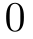
\includegraphics[width=9.04pt]{images-full/p034-i010.png}}\allowbreak{} 的$n$ 阶方阵，则
\sourceblock{396.06}{images-full/p034-d005.png}
注意到
\sourceblock{114.69}{images-full/p034-d006.png}
\sourceblock{341.82}{images-full/p034-d007.png}
\sourceblock{143.51}{images-full/p034-d008.png}
另一方面，若\allowbreak{}\raisebox{-2.88pt}{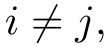
\includegraphics[width=29.31pt]{images-full/p034-i012.png}}\allowbreak{}则\allowbreak{}\raisebox{-2.88pt}{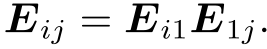
\includegraphics[width=75.01pt]{images-full/p034-i013.png}}\allowbreak{} 从而


% SOURCE_PDF_PAGE 35

\hypertarget{source-p035}{}
\sourceblock{370.07}{images-full/p035-d000.png}
所以，对任意\allowbreak{}\raisebox{-3.12pt}{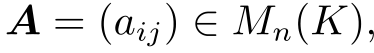
\includegraphics[width=105.32pt]{images-full/p035-i000.png}}\allowbreak{}，有
\sourceblock{362.16}{images-full/p035-d001.png}
\par\medskip\noindent\textbf{【例1.2.29 】设$A$ 为$n$ 阶实矩阵，且$E-A$ 的特征值的模均小于1.证明\allowbreak{}\raisebox{-2.28pt}{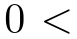
\includegraphics[width=21.47pt]{images-full/p035-i004.png}}\allowbreak{}}
\sourceblock{49.15}{images-full/p035-d002.png}
\par\noindent\textbf{证明}\ 设$A$ 的复特征值为机\allowbreak{}\raisebox{-2.76pt}{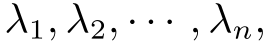
\includegraphics[width=73.97pt]{images-full/p035-i006.png}}\allowbreak{}，则$E-A$ 的特征值为\allowbreak{}\raisebox{-2.76pt}{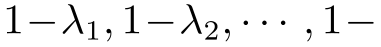
\includegraphics[width=107.35pt]{images-full/p035-i008.png}}\allowbreak{}
\allowbreak{}\raisebox{-2.64pt}{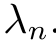
\includegraphics[width=15.44pt]{images-full/p035-i009.png}}\allowbreak{}.故对任意$i$，
\sourceblock{63.84}{images-full/p035-d003.png}
若\allowbreak{}\raisebox{-2.76pt}{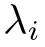
\includegraphics[width=12.43pt]{images-full/p035-i011.png}}\allowbreak{} 为实数，由\allowbreak{}\raisebox{-2.88pt}{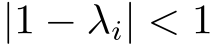
\includegraphics[width=61.02pt]{images-full/p035-i012.png}}\allowbreak{} 得\allowbreak{}\raisebox{-2.76pt}{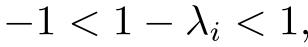
\includegraphics[width=86.65pt]{images-full/p035-i013.png}}\allowbreak{}，即\allowbreak{}\raisebox{-2.76pt}{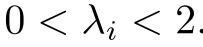
\includegraphics[width=57.11pt]{images-full/p035-i014.png}}\allowbreak{}.
若\allowbreak{}\raisebox{-2.64pt}{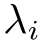
\includegraphics[width=12.43pt]{images-full/p035-i015.png}}\allowbreak{}为非实数，则\allowbreak{}\raisebox{-3.12pt}{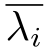
\includegraphics[width=14.12pt]{images-full/p035-i016.png}}\allowbreak{}也是$A$ 的特征值.此时
\sourceblock{200.57}{images-full/p035-d004.png}
这时
\sourceblock{91.53}{images-full/p035-d005.png}
由\allowbreak{}\raisebox{-3.00pt}{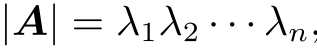
\includegraphics[width=89.12pt]{images-full/p035-i018.png}}\allowbreak{}可得\allowbreak{}\raisebox{-3.00pt}{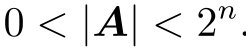
\includegraphics[width=69.07pt]{images-full/p035-i019.png}}\allowbreak{} 口
\par\medskip\noindent\textbf{【例1.2.30 】设\allowbreak{}\raisebox{-2.76pt}{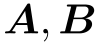
\includegraphics[width=28.81pt]{images-full/p035-i020.png}}\allowbreak{} 分别为$m$ 阶和$n$ 阶方阵，$C$ 为\allowbreak{}\raisebox{-1.80pt}{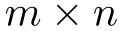
\includegraphics[width=34.46pt]{images-full/p035-i024.png}}\allowbreak{} 矩阵，且满足}
\sourceblock{144.64}{images-full/p035-d006.png}
\par\noindent\textbf{证明}\ $A$ 与$B$ 至少有\allowbreak{}\raisebox{-1.68pt}{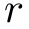
\includegraphics[width=7.91pt]{images-full/p035-i027.png}}\allowbreak{}个相同的特征值(包括重数).
\par\noindent\textbf{证明}\ 由于\allowbreak{}\raisebox{-3.00pt}{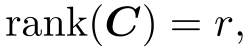
\includegraphics[width=68.62pt]{images-full/p035-i028.png}}\allowbreak{}故存在$m$ 阶可逆矩阵\allowbreak{}\raisebox{-2.76pt}{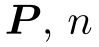
\includegraphics[width=27.68pt]{images-full/p035-i030.png}}\allowbreak{} 阶可逆矩阵$Q$，使得
\sourceblock{120.91}{images-full/p035-d007.png}
由\allowbreak{}\raisebox{-2.28pt}{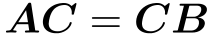
\includegraphics[width=60.45pt]{images-full/p035-i032.png}}\allowbreak{} 得到
\sourceblock{277.41}{images-full/p035-d008.png}
即
\sourceblock{358.21}{images-full/p035-d009.png}


% SOURCE_PDF_PAGE 36

\hypertarget{source-p036}{}
\sourceblock{245.77}{images-full/p036-d000.png}
令
\sourceblock{435.05}{images-full/p036-d001.png}
\sourceblock{389.85}{images-full/p036-d002.png}
这里用到\allowbreak{}\raisebox{-2.64pt}{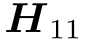
\includegraphics[width=23.73pt]{images-full/p036-i000.png}}\allowbreak{}有$T$ 个特征值，这对任意数域不一定成立.但显然复数域上的矩阵
\allowbreak{}\raisebox{-2.64pt}{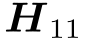
\includegraphics[width=23.73pt]{images-full/p036-i002.png}}\allowbreak{} 的$T$个特征值是$H$ 与$T$ 的公共特征值.注意到$A$ 与$H$ 相似，$B$ 与$T$ 相似.故
$A$ 与$H$ 有相同的特征值，$B$ 与$T$ 有相同的特征值.因此$A$ 与$B$ 至少有$T$个相同的特
征值.口
园也型λ悦和等支挤在帕
此类型题目通常考察下面内容:
\par\noindent (1) 利用分块初等变换进行降阶计算.
\par\noindent (2) 初等矩阵与初等变换的关系.
\par\noindent (3) 分块矩阵的性质及其计算.
解题中熟记下列基本结果是有帮助的:
\sourceblock{210.74}{images-full/p036-d003.png}


% SOURCE_PDF_PAGE 37

\hypertarget{source-p037}{}
\sourceblock{210.18}{images-full/p037-d000.png}
\sourceblock{394.37}{images-full/p037-d001.png}
所以
\sourceblock{300.01}{images-full/p037-d002.png}
故
\sourceblock{409.62}{images-full/p037-d003.png}
由
\sourceblock{344.65}{images-full/p037-d004.png}
\sourceblock{378.55}{images-full/p037-d005.png}
\sourceblock{304.53}{images-full/p037-d006.png}
\sourceblock{450.00}{images-full/p037-d007.png}
\par\noindent\textbf{证明}\ 对矩阵$Q$ 施行分块初等变换
\sourceblock{206.79}{images-full/p037-d008.png}
\sourceblock{380.24}{images-full/p037-d009.png}


% SOURCE_PDF_PAGE 38

\hypertarget{source-p038}{}
于是\allowbreak{}\raisebox{-3.36pt}{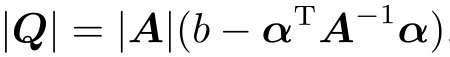
\includegraphics[width=127.04pt]{images-full/p038-i000.png}}\allowbreak{}，由于\allowbreak{}\raisebox{-3.00pt}{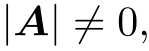
\includegraphics[width=42.01pt]{images-full/p038-i001.png}}\allowbreak{}，故
\sourceblock{293.80}{images-full/p038-d000.png}
\par\medskip\noindent\textbf{【例1.2.32 】设$A$ 为$m$ 阶可逆矩阵，$B$ 为\allowbreak{}\raisebox{-1.80pt}{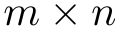
\includegraphics[width=34.46pt]{images-full/p038-i005.png}}\allowbreak{} 矩阵，$C$ 为\allowbreak{}\raisebox{-1.80pt}{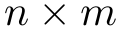
\includegraphics[width=34.46pt]{images-full/p038-i007.png}}\allowbreak{} 矩阵，$D$ 为}
$n$阶方阵.证明
\sourceblock{174.58}{images-full/p038-d001.png}
\par\noindent\textbf{证明}\ 困
\sourceblock{381.94}{images-full/p038-d002.png}
进一步地，若\allowbreak{}\raisebox{-2.76pt}{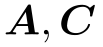
\includegraphics[width=28.81pt]{images-full/p038-i010.png}}\allowbreak{} 可交换，则
\sourceblock{353.12}{images-full/p038-d003.png}
【注1.2.7】此例中，若$D$ 也可逆，则杳
\sourceblock{207.35}{images-full/p038-d004.png}
从而
\sourceblock{166.67}{images-full/p038-d005.png}
由此得到
\sourceblock{207.92}{images-full/p038-d006.png}
以\allowbreak{}\raisebox{-2.28pt}{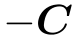
\includegraphics[width=22.03pt]{images-full/p038-i012.png}}\allowbreak{}代替上式中的$C$ 可得
\sourceblock{207.92}{images-full/p038-d007.png}
这个等式也称为行列式的降阶公式.
特别地，若取\allowbreak{}\raisebox{-2.76pt}{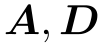
\includegraphics[width=29.38pt]{images-full/p038-i014.png}}\allowbreak{} 为单位矩阵，则有\allowbreak{}\raisebox{-3.00pt}{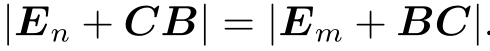
\includegraphics[width=138.14pt]{images-full/p038-i015.png}}\allowbreak{}


% SOURCE_PDF_PAGE 39

\hypertarget{source-p039}{}
\par\medskip\noindent\textbf{【例1.2.33 】设\allowbreak{}\raisebox{-2.76pt}{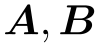
\includegraphics[width=28.81pt]{images-full/p039-i000.png}}\allowbreak{} 为$n$ 阶矩阵证明}
\sourceblock{250.29}{images-full/p039-d000.png}
\sourceblock{405.10}{images-full/p039-d001.png}
所以
\sourceblock{436.18}{images-full/p039-d002.png}
(方法2) 直接利用关于矩阵秩的不等式，得
\sourceblock{362.73}{images-full/p039-d003.png}
\par\medskip\noindent\textbf{【例1.2.34】令}
\sourceblock{243.51}{images-full/p039-d004.png}
求\allowbreak{}\raisebox{-3.00pt}{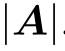
\includegraphics[width=18.15pt]{images-full/p039-i002.png}}\allowbreak{}
解易知
\sourceblock{249.73}{images-full/p039-d005.png}
\sourceblock{317.53}{images-full/p039-d006.png}


% SOURCE_PDF_PAGE 40

\hypertarget{source-p040}{}
\sourceblock{267.24}{images-full/p040-d000.png}
\par\medskip\noindent\textbf{【例1.2.36 】设\allowbreak{}\raisebox{-2.76pt}{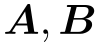
\includegraphics[width=28.81pt]{images-full/p041-i000.png}}\allowbreak{} 均为\allowbreak{}\raisebox{-1.68pt}{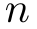
\includegraphics[width=10.17pt]{images-full/p041-i001.png}}\allowbreak{} 阶实矩阵，证明}
\sourceblock{202.83}{images-full/p041-d001.png}
\par\noindent\textbf{证明}\ 困为
\sourceblock{406.23}{images-full/p041-d002.png}
\sourceblock{181.36}{images-full/p041-d003.png}
进一步地，
\sourceblock{329.96}{images-full/p041-d004.png}
\sourceblock{108.48}{images-full/p041-d005.png}
\sourceblock{262.16}{images-full/p041-d006.png}


% SOURCE_PDF_PAGE 42

\hypertarget{source-p042}{}
解注意到
\sourceblock{262.72}{images-full/p042-d000.png}
\sourceblock{450.00}{images-full/p042-d001.png}
\sourceblock{392.67}{images-full/p042-d002.png}
\par\noindent (2) 求满足\allowbreak{}\raisebox{-2.28pt}{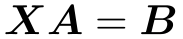
\includegraphics[width=51.41pt]{images-full/p042-i000.png}}\allowbreak{} 的所杳三阶矩阵\allowbreak{}\raisebox{-2.28pt}{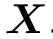
\includegraphics[width=14.63pt]{images-full/p042-i001.png}}\allowbreak{}


% SOURCE_PDF_PAGE 43

\hypertarget{source-p043}{}
\sourceblock{374.59}{images-full/p043-d000.png}
\sourceblock{385.33}{images-full/p043-d001.png}
\sourceblock{290.97}{images-full/p043-d002.png}
\sourceblock{322.05}{images-full/p043-d003.png}


% SOURCE_PDF_PAGE 44

\hypertarget{source-p044}{}
从而
\sourceblock{450.00}{images-full/p044-d000.png}
\sourceblock{445.22}{images-full/p044-d001.png}
对右边直接计算得
\sourceblock{282.50}{images-full/p044-d002.png}
所以
\sourceblock{339.56}{images-full/p044-d003.png}


% SOURCE_PDF_PAGE 45

\hypertarget{source-p045}{}
园也型々t.'tiJð-创刊的制确定
\par\medskip\noindent\textbf{【例1.2.41 】设$B$ 为$p$ 阶复方阵，}
\sourceblock{184.19}{images-full/p046-d000.png}
试求$B$ 的初等因子.
解显然，$B$ 的特征多项式为\allowbreak{}\raisebox{-3.00pt}{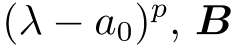
\includegraphics[width=66.53pt]{images-full/p046-i004.png}}\allowbreak{} 的特征值都等于\allowbreak{}\raisebox{-2.04pt}{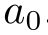
\includegraphics[width=13.52pt]{images-full/p046-i005.png}}\allowbreak{}.
\par\noindent (1) 当\allowbreak{}\raisebox{-2.76pt}{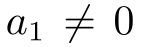
\includegraphics[width=39.55pt]{images-full/p046-i006.png}}\allowbreak{} 时，\allowbreak{}\raisebox{-3.00pt}{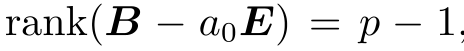
\includegraphics[width=130.73pt]{images-full/p046-i007.png}}\allowbreak{}，特征值\allowbreak{}\raisebox{-2.04pt}{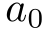
\includegraphics[width=13.56pt]{images-full/p046-i008.png}}\allowbreak{} 的儿何重数为1.故$B$ 的
Jordan 标准形中只能有一个Jordan 块，即$B$ 只有一个初等因子\allowbreak{}\raisebox{-3.00pt}{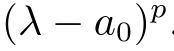
\includegraphics[width=48.79pt]{images-full/p046-i011.png}}\allowbreak{}.
\par\noindent (2) 当\allowbreak{}\raisebox{-2.88pt}{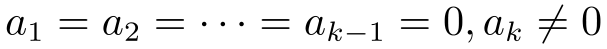
\includegraphics[width=171.19pt]{images-full/p046-i012.png}}\allowbreak{} 时，为找出$B$ 的所有初等因子，我们先来确
定$B$ 的Jordan 标准形中Jordan 块的形状和个数.
注意到
\sourceblock{362.73}{images-full/p046-d001.png}
\par \allowbreak{}\raisebox{-3.48pt}{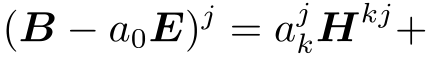
\includegraphics[width=121.47pt]{images-full/p046-i015.png}}\allowbreak{}若干$H$ 的更高罪次项.
所以
\sourceblock{331.65}{images-full/p046-d002.png}
记\allowbreak{}\raisebox{-3.00pt}{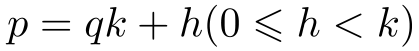
\includegraphics[width=118.08pt]{images-full/p046-i017.png}}\allowbreak{}(带余除法) ，则
\sourceblock{269.50}{images-full/p046-d003.png}
现假设$B$ 的初等因子有\allowbreak{}\raisebox{-2.16pt}{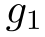
\includegraphics[width=12.43pt]{images-full/p046-i019.png}}\allowbreak{}个\allowbreak{}\raisebox{-2.88pt}{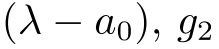
\includegraphics[width=61.58pt]{images-full/p046-i020.png}}\allowbreak{} 个\allowbreak{}\raisebox{-3.36pt}{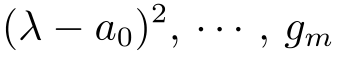
\includegraphics[width=95.48pt]{images-full/p046-i021.png}}\allowbreak{} 个\allowbreak{}\raisebox{-3.00pt}{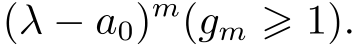
\includegraphics[width=99.82pt]{images-full/p046-i022.png}}\allowbreak{}
对此$B$ 有相应的Jordan 标准形.从$B$ 的这个Jordan 标准形又可定义出各个\allowbreak{}\raisebox{-3.00pt}{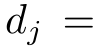
\includegraphics[width=27.68pt]{images-full/p046-i025.png}}\allowbreak{}


% SOURCE_PDF_PAGE 47

\hypertarget{source-p047}{}
\allowbreak{}\raisebox{-3.24pt}{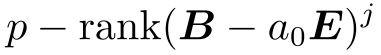
\includegraphics[width=107.35pt]{images-full/p047-i000.png}}\allowbreak{} 的值:
\sourceblock{190.97}{images-full/p047-d000.png}
将这组\allowbreak{}\raisebox{-3.00pt}{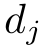
\includegraphics[width=12.99pt]{images-full/p047-i001.png}}\allowbreak{}的值与前面己经得到的值进行比较，可得
\sourceblock{214.13}{images-full/p047-d001.png}
\sourceblock{303.40}{images-full/p047-d002.png}
所以当\allowbreak{}\raisebox{-2.88pt}{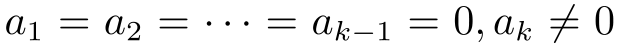
\includegraphics[width=175.15pt]{images-full/p047-i002.png}}\allowbreak{} 时$B$ 的初等因子有:$k-h$ 个\allowbreak{}\raisebox{-3.00pt}{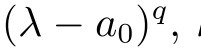
\includegraphics[width=56.54pt]{images-full/p047-i005.png}}\allowbreak{}h 个
\allowbreak{}\raisebox{-3.24pt}{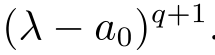
\includegraphics[width=60.51pt]{images-full/p047-i006.png}}\allowbreak{}
\par\noindent (3) 最后，显然当\allowbreak{}\raisebox{-2.88pt}{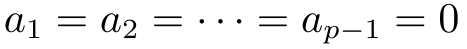
\includegraphics[width=131.64pt]{images-full/p047-i007.png}}\allowbreak{} 时，$B$ 有$p$ 个初等因子，它们都是\allowbreak{}\raisebox{-2.76pt}{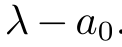
\includegraphics[width=34.42pt]{images-full/p047-i010.png}}\allowbreak{}.
困县型八州树例削
\par\medskip\noindent\textbf{【例1.2.42 】设\allowbreak{}\raisebox{-1.68pt}{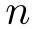
\includegraphics[width=10.17pt]{images-full/p047-i011.png}}\allowbreak{} 阶实方阵\allowbreak{}\raisebox{-2.76pt}{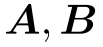
\includegraphics[width=28.81pt]{images-full/p047-i012.png}}\allowbreak{} 满足\allowbreak{}\raisebox{-3.00pt}{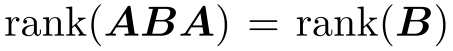
\includegraphics[width=127.69pt]{images-full/p047-i013.png}}\allowbreak{} 证明:\allowbreak{}\raisebox{-2.28pt}{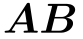
\includegraphics[width=23.16pt]{images-full/p047-i014.png}}\allowbreak{} 与}
\allowbreak{}\raisebox{-2.28pt}{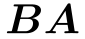
\includegraphics[width=23.73pt]{images-full/p047-i015.png}}\allowbreak{} 相似.
\par\noindent\textbf{证明}\ 设\allowbreak{}\raisebox{-3.00pt}{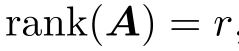
\includegraphics[width=67.18pt]{images-full/p047-i016.png}}\allowbreak{}，且设
\sourceblock{373.46}{images-full/p047-d003.png}
\sourceblock{301.14}{images-full/p047-d004.png}


% SOURCE_PDF_PAGE 48

\hypertarget{source-p048}{}
\sourceblock{323.74}{images-full/p048-d000.png}
\sourceblock{298.88}{images-full/p048-d001.png}
从而有
\sourceblock{372.90}{images-full/p048-d002.png}
【点i平】此题表面上看是矩阵相似的判定问题，实质是矩阵的等价标准形的应用.当
然也还需要利用分块矩阵技巧.
\sourceblock{450.00}{images-full/p048-d003.png}


% SOURCE_PDF_PAGE 49

\hypertarget{source-p049}{}
如秩、迹、行列式、特征值等.此外，不变因子组和初等因子组也都是矩阵的相似不变量，
而且由于初等因子组唯一地决定了Jor也且标准形，从而$A$ 与$B$ 相似又等价于$A$ 与$B$
杳相同的初等因子组，也等价于$A$与$B$ 有相同的不变因子组.
\par\medskip\noindent\textbf{【例1.2.44 】设实对称矩阵}
\sourceblock{98.87}{images-full/p049-d000.png}
\sourceblock{280.80}{images-full/p049-d001.png}
相似，求\allowbreak{}\raisebox{-2.16pt}{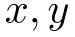
\includegraphics[width=20.90pt]{images-full/p049-i006.png}}\allowbreak{} 及满足\allowbreak{}\raisebox{-3.24pt}{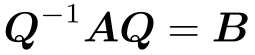
\includegraphics[width=71.75pt]{images-full/p049-i007.png}}\allowbreak{} 的正交矩阵\allowbreak{}\raisebox{-2.76pt}{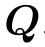
\includegraphics[width=12.65pt]{images-full/p049-i008.png}}\allowbreak{}
解$A$ 与$B$ 相似=\allowbreak{}\raisebox{-2.40pt}{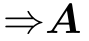
\includegraphics[width=24.86pt]{images-full/p049-i011.png}}\allowbreak{} 与$B$ 有相同的迹和行列式.进而得
\sourceblock{128.25}{images-full/p049-d002.png}
\sourceblock{428.27}{images-full/p049-d003.png}


% SOURCE_PDF_PAGE 50

\hypertarget{source-p050}{}
\sourceblock{393.24}{images-full/p050-d000.png}
\sourceblock{276.85}{images-full/p050-d001.png}
\sourceblock{397.19}{images-full/p050-d002.png}
\sourceblock{436.74}{images-full/p050-d003.png}
C 使得$A$ 相似于
\sourceblock{110.74}{images-full/p050-d004.png}
\par\noindent\textbf{证明}\ (1) 由署等阵可对角化，且其特征值\allowbreak{}\raisebox{-2.76pt}{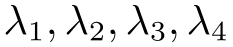
\includegraphics[width=65.54pt]{images-full/p050-i001.png}}\allowbreak{} 要么为1，要么为0，因此有
\sourceblock{146.90}{images-full/p050-d005.png}


% SOURCE_PDF_PAGE 51

\hypertarget{source-p051}{}
\sourceblock{266.11}{images-full/p051-d000.png}
\sourceblock{450.00}{images-full/p051-d001.png}
\sourceblock{298.88}{images-full/p051-d002.png}
考察关于句\allowbreak{}\raisebox{-2.04pt}{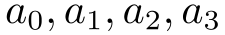
\includegraphics[width=63.28pt]{images-full/p051-i000.png}}\allowbreak{}的线性方程组:
\sourceblock{428.83}{images-full/p051-d003.png}
\sourceblock{159.33}{images-full/p051-d004.png}
则有\allowbreak{}\raisebox{-3.00pt}{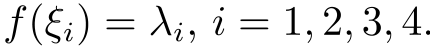
\includegraphics[width=121.02pt]{images-full/p051-i001.png}}\allowbreak{} 所以
\sourceblock{398.32}{images-full/p051-d005.png}
\sourceblock{383.07}{images-full/p051-d006.png}


% SOURCE_PDF_PAGE 52

\hypertarget{source-p052}{}
因此本题获证.口
\phantomsection\addcontentsline{toc}{section}{1.3 真题选讲与点评}
\par 4 u 真题选讲与点评\}-
\par\medskip\noindent\textbf{【例1.3.1 】(第四届全国初赛题{\symbolfont ①})已知实矩阵}
\sourceblock{185.88}{images-full/p053-d002.png}
\sourceblock{447.48}{images-full/p053-d003.png}
\par\noindent\textbf{证明}\ (l)\allowbreak{}\raisebox{-2.28pt}{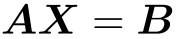
\includegraphics[width=50.28pt]{images-full/p053-i005.png}}\allowbreak{} 有解等价于$B$ 的列向量组可由$A$ 的列向量组线性表示. \allowbreak{}\raisebox{-2.28pt}{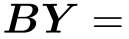
\includegraphics[width=36.16pt]{images-full/p053-i008.png}}\allowbreak{}
$A$无解等价于$A$ 的某个列向量不能由$B$ 的列向量组线性表示.对\allowbreak{}\raisebox{-3.00pt}{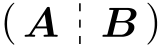
\includegraphics[width=46.33pt]{images-full/p053-i012.png}}\allowbreak{} 作初等变换
\sourceblock{311.31}{images-full/p053-d004.png}
\sourceblock{371.77}{images-full/p053-d005.png}
{\symbolfont ①}第四届全国太学生数学竞赛初赛数学专业组试题简写为第四届全国初赛题.以下为方便叙述，数学专业组试题全部
按这种格式简写，非数学专业组试题按照第四届全国初赛题(非数学类)的格式标记.


% SOURCE_PDF_PAGE 54

\hypertarget{source-p054}{}
而若\allowbreak{}\raisebox{-2.88pt}{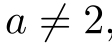
\includegraphics[width=31.21pt]{images-full/p054-i000.png}}\allowbreak{}，则$A$ 的列向量组线性无关.$B$ 的两个列向量都可以由$A$ 的列向量组线
性表示.所以\allowbreak{}\raisebox{-2.28pt}{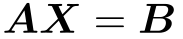
\includegraphics[width=51.41pt]{images-full/p054-i004.png}}\allowbreak{}有解的充要条件是\allowbreak{}\raisebox{-2.76pt}{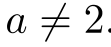
\includegraphics[width=31.03pt]{images-full/p054-i005.png}}\allowbreak{}
类似地，对\allowbreak{}\raisebox{-3.00pt}{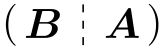
\includegraphics[width=46.89pt]{images-full/p054-i006.png}}\allowbreak{}作初等变换
\sourceblock{450.00}{images-full/p054-d000.png}
\allowbreak{}\raisebox{-3.00pt}{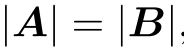
\includegraphics[width=51.64pt]{images-full/p054-i007.png}}\allowbreak{}，即
\sourceblock{176.84}{images-full/p054-d001.png}
\sourceblock{323.18}{images-full/p054-d002.png}
$A$ 和$B$ 的特征多项式均为\allowbreak{}\raisebox{-3.12pt}{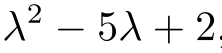
\includegraphics[width=62.38pt]{images-full/p054-i010.png}}\allowbreak{}，它有两个互不相等的实根\allowbreak{}\raisebox{-2.76pt}{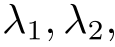
\includegraphics[width=32.29pt]{images-full/p054-i011.png}}\allowbreak{}，所以$A$ 与$B$
\sourceblock{450.00}{images-full/p054-d003.png}
\sourceblock{265.55}{images-full/p054-d004.png}
所以\allowbreak{}\raisebox{-3.00pt}{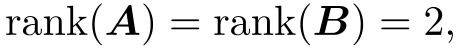
\includegraphics[width=128.49pt]{images-full/p054-i014.png}}\allowbreak{}，且$A$ 的正负惯性指数也都是1.
易知$A$ 的一个合同标准形为
\sourceblock{450.00}{images-full/p054-d005.png}


% SOURCE_PDF_PAGE 55

\hypertarget{source-p055}{}
\par\medskip\noindent\textbf{【例1.3.2 】(第七届全国初赛题)设$A$ 为$n$ 阶方阵其$n$个特征值均为偶数. 证明}
关于$X$ 的矩阵方程
\sourceblock{119.78}{images-full/p055-d000.png}
\sourceblock{209.05}{images-full/p055-d001.png}
\sourceblock{104.52}{images-full/p055-d002.png}
设\allowbreak{}\raisebox{-3.24pt}{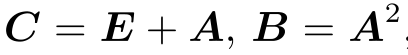
\includegraphics[width=115.05pt]{images-full/p055-i004.png}}\allowbreak{}，且$A$ 的$n$个特征值为\allowbreak{}\raisebox{-2.76pt}{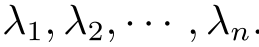
\includegraphics[width=72.78pt]{images-full/p055-i007.png}}\allowbreak{} 则$C$ 的$n$个特征
值为
\sourceblock{136.73}{images-full/p055-d003.png}
$B$ 的$n$个特征值为
\sourceblock{310.18}{images-full/p055-d004.png}
\sourceblock{311.31}{images-full/p055-d005.png}
以此类推.对任意的正整数$k$ 有\allowbreak{}\raisebox{-2.88pt}{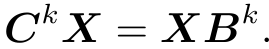
\includegraphics[width=75.52pt]{images-full/p055-i013.png}}\allowbreak{}•
设$C$ 的特征多项式为
\sourceblock{406.80}{images-full/p055-d006.png}
\sourceblock{216.96}{images-full/p055-d007.png}
\sourceblock{154.81}{images-full/p055-d008.png}
由于\allowbreak{}\raisebox{-3.24pt}{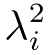
\includegraphics[width=14.12pt]{images-full/p055-i015.png}}\allowbreak{} 为偶数，\allowbreak{}\raisebox{-3.00pt}{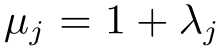
\includegraphics[width=62.71pt]{images-full/p055-i016.png}}\allowbreak{} 为奇数.所以\allowbreak{}\raisebox{-3.00pt}{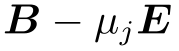
\includegraphics[width=50.28pt]{images-full/p055-i017.png}}\allowbreak{} 的特征值均不等于\allowbreak{}\raisebox{-2.28pt}{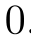
\includegraphics[width=8.43pt]{images-full/p055-i018.png}}\allowbreak{}. 故\allowbreak{}\raisebox{-3.00pt}{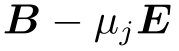
\includegraphics[width=50.28pt]{images-full/p055-i019.png}}\allowbreak{}
可逆.由此得到\allowbreak{}\raisebox{-2.40pt}{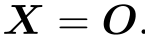
\includegraphics[width=40.63pt]{images-full/p055-i020.png}}\allowbreak{}口
\par\medskip\noindent\textbf{【例1.3.31 (第八届全国初赛题)设\allowbreak{}\raisebox{-2.76pt}{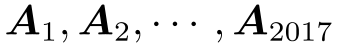
\includegraphics[width=95.48pt]{images-full/p055-i021.png}}\allowbreak{} 为2016 阶实方阵证明: 关}
于\allowbreak{}\raisebox{-2.16pt}{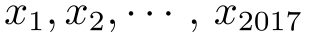
\includegraphics[width=87.01pt]{images-full/p055-i022.png}}\allowbreak{} 的方程
\sourceblock{218.09}{images-full/p055-d009.png}


% SOURCE_PDF_PAGE 56

\hypertarget{source-p056}{}
至少有一组非零实数解，其中det 表示行列式.
\sourceblock{389.85}{images-full/p056-d000.png}
\sourceblock{208.48}{images-full/p056-d001.png}
这个方程组有2016 个方程、2017 个未知数.所以它有非零解.设\allowbreak{}\raisebox{-2.16pt}{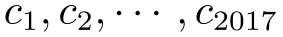
\includegraphics[width=79.66pt]{images-full/p056-i000.png}}\allowbreak{} 是它的
一组非零解.这表明
\sourceblock{163.28}{images-full/p056-d002.png}
的第\allowbreak{}\raisebox{-2.28pt}{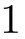
\includegraphics[width=6.78pt]{images-full/p056-i001.png}}\allowbreak{}列为零向量.从而
\sourceblock{215.83}{images-full/p056-d003.png}
故\allowbreak{}\raisebox{-2.04pt}{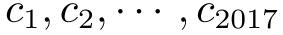
\includegraphics[width=79.66pt]{images-full/p056-i002.png}}\allowbreak{} 是方程
\sourceblock{218.09}{images-full/p056-d004.png}
的一组非零实数解.口
\par\medskip\noindent\textbf{【例1.3.4】(第九届全国初赛题)设\allowbreak{}\raisebox{-3.12pt}{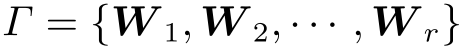
\includegraphics[width=131.64pt]{images-full/p056-i003.png}}\allowbreak{} 为$T$个互不相同的可}
逆$n$阶复方阵构成的集合若该集合关于矩阵乘法封闭(即\allowbreak{}\raisebox{-2.76pt}{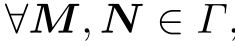
\includegraphics[width=66.14pt]{images-full/p056-i006.png}}\allowbreak{}，有\allowbreak{}\raisebox{-2.97pt}{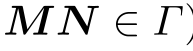
\includegraphics[width=54.36pt]{images-full/p056-i007.png}}\allowbreak{}.
\par\noindent\textbf{证明}\ 
\sourceblock{206.22}{images-full/p056-d005.png}
\sourceblock{361.03}{images-full/p056-d006.png}
\sourceblock{218.09}{images-full/p056-d007.png}
又\allowbreak{}\raisebox{-2.28pt}{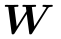
\includegraphics[width=16.95pt]{images-full/p056-i008.png}}\allowbreak{} 可逆，若研rwi=wwj ，则奋阴气=Wj . 这表明\allowbreak{}\raisebox{-2.28pt}{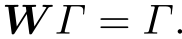
\includegraphics[width=51.03pt]{images-full/p056-i009.png}}\allowbreak{}.
\sourceblock{235.04}{images-full/p056-d008.png}
\sourceblock{257.64}{images-full/p056-d009.png}
即\allowbreak{}\raisebox{-2.88pt}{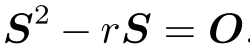
\includegraphics[width=70.26pt]{images-full/p056-i010.png}}\allowbreak{} 若\allowbreak{}\raisebox{-2.28pt}{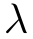
\includegraphics[width=9.04pt]{images-full/p056-i011.png}}\allowbreak{} 为$S$ 的一个特征值，则有\allowbreak{}\raisebox{-2.76pt}{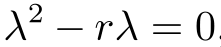
\includegraphics[width=62.07pt]{images-full/p056-i013.png}}\allowbreak{}，即\allowbreak{}\raisebox{-2.28pt}{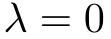
\includegraphics[width=31.07pt]{images-full/p056-i014.png}}\allowbreak{} 或\allowbreak{}\raisebox{-2.28pt}{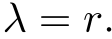
\includegraphics[width=31.43pt]{images-full/p056-i015.png}}\allowbreak{}.这表明
$S$ 的特征值只可能为0 或\allowbreak{}\raisebox{-1.56pt}{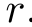
\includegraphics[width=8.72pt]{images-full/p056-i017.png}}\allowbreak{}


% SOURCE_PDF_PAGE 57

\hypertarget{source-p057}{}
\sourceblock{450.00}{images-full/p057-d000.png}
\par\medskip\noindent\textbf{【例1.3.5] (第九届全国初赛题)给定非霉实数\allowbreak{}\raisebox{-1.56pt}{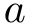
\includegraphics[width=9.04pt]{images-full/p057-i000.png}}\allowbreak{} 及\allowbreak{}\raisebox{-1.56pt}{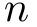
\includegraphics[width=10.17pt]{images-full/p057-i001.png}}\allowbreak{} 阶实反对称矩阵A. 记}
\sourceblock{250.29}{images-full/p057-d001.png}
\par\noindent\textbf{证明}\ 任取$T$ 中两个元素\allowbreak{}\raisebox{-2.88pt}{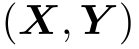
\includegraphics[width=38.98pt]{images-full/p057-i003.png}}\allowbreak{} 和\allowbreak{}\raisebox{-3.00pt}{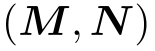
\includegraphics[width=43.50pt]{images-full/p057-i004.png}}\allowbreak{} 必有
\sourceblock{110.74}{images-full/p057-d002.png}
\par\noindent\textbf{证明}\ 反证法.若存在\allowbreak{}\raisebox{-3.00pt}{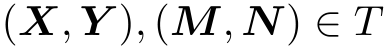
\includegraphics[width=110.17pt]{images-full/p057-i005.png}}\allowbreak{}使得
\sourceblock{110.74}{images-full/p057-d003.png}
则有
\sourceblock{110.74}{images-full/p057-d004.png}
因为\allowbreak{}\raisebox{-3.36pt}{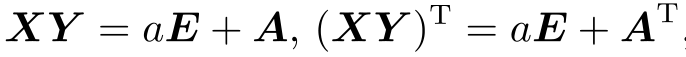
\includegraphics[width=193.69pt]{images-full/p057-i006.png}}\allowbreak{}，又\allowbreak{}\raisebox{-3.24pt}{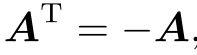
\includegraphics[width=55.36pt]{images-full/p057-i007.png}}\allowbreak{}，所以
\sourceblock{120.34}{images-full/p057-d005.png}
\sourceblock{268.38}{images-full/p057-d006.png}
因此
\sourceblock{378.55}{images-full/p057-d007.png}
\sourceblock{331.65}{images-full/p057-d008.png}
\sourceblock{450.00}{images-full/p057-d009.png}
\allowbreak{}\raisebox{-2.76pt}{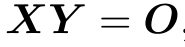
\includegraphics[width=52.04pt]{images-full/p057-i008.png}}\allowbreak{}，与\allowbreak{}\raisebox{-2.76pt}{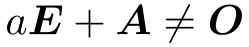
\includegraphics[width=70.06pt]{images-full/p057-i009.png}}\allowbreak{} 矛盾.口


% SOURCE_PDF_PAGE 58

\hypertarget{source-p058}{}
\par\medskip\noindent\textbf{【例1.3.6】(第八届全国初赛题)设$n$ 为奇数，\allowbreak{}\raisebox{-2.76pt}{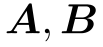
\includegraphics[width=28.81pt]{images-full/p058-i001.png}}\allowbreak{} 为两个$n$阶实方阵且\allowbreak{}\raisebox{-2.40pt}{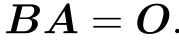
\includegraphics[width=50.29pt]{images-full/p058-i003.png}}\allowbreak{}}
记\allowbreak{}\raisebox{-2.64pt}{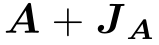
\includegraphics[width=44.63pt]{images-full/p058-i004.png}}\allowbreak{} 的特征值集舍为\allowbreak{}\raisebox{-2.64pt}{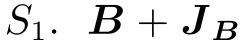
\includegraphics[width=68.93pt]{images-full/p058-i005.png}}\allowbreak{} 的特征值集合为\allowbreak{}\raisebox{-2.76pt}{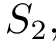
\includegraphics[width=15.61pt]{images-full/p058-i006.png}}\allowbreak{}其中\allowbreak{}\raisebox{-2.76pt}{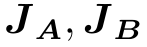
\includegraphics[width=41.24pt]{images-full/p058-i007.png}}\allowbreak{} 分别表示
\allowbreak{}\raisebox{-2.76pt}{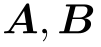
\includegraphics[width=28.25pt]{images-full/p058-i008.png}}\allowbreak{} 的Jordan 标准形.证明:\allowbreak{}\raisebox{-2.64pt}{\includegraphics[width=61.28pt]{images-full/p058-i009.png}}\allowbreak{}.
\par\noindent\textbf{证明}\ \allowbreak{}\raisebox{-2.76pt}{\includegraphics[width=61.61pt]{images-full/p058-i010.png}}\allowbreak{}，即\allowbreak{}\raisebox{-2.28pt}{\includegraphics[width=9.04pt]{images-full/p058-i011.png}}\allowbreak{} 为\allowbreak{}\raisebox{-2.76pt}{\includegraphics[width=43.50pt]{images-full/p058-i012.png}}\allowbreak{} 或者\allowbreak{}\raisebox{-2.64pt}{\includegraphics[width=44.63pt]{images-full/p058-i013.png}}\allowbreak{} 的特征值或等价地\allowbreak{}\raisebox{-2.76pt}{\includegraphics[width=43.50pt]{images-full/p058-i014.png}}\allowbreak{} 或者
\sourceblock{345.78}{images-full/p058-d000.png}
\sourceblock{276.28}{images-full/p058-d001.png}
\sourceblock{433.92}{images-full/p058-d002.png}
\sourceblock{276.28}{images-full/p058-d003.png}
解对$B$ 进行初等变换:
\sourceblock{262.72}{images-full/p058-d004.png}
\sourceblock{330.52}{images-full/p058-d005.png}
注意到$A$ 是可逆反对称矩阵，故有
\sourceblock{224.87}{images-full/p058-d006.png}
\sourceblock{368.38}{images-full/p058-d007.png}
由此得\allowbreak{}\raisebox{-3.24pt}{\includegraphics[width=75.28pt]{images-full/p058-i017.png}}\allowbreak{}，故\allowbreak{}\raisebox{-3.00pt}{\includegraphics[width=69.58pt]{images-full/p058-i018.png}}\allowbreak{}
【点评】此题考察的是矩阵秩的计算问题.由于$B$ 是分块形式，因此使用分块初等
变换是自然的.
\par\medskip\noindent\textbf{【例1.3.8] (第二届全国决赛题)设\allowbreak{}\raisebox{-3.12pt}{\includegraphics[width=87.57pt]{images-full/p058-i020.png}}\allowbreak{}是数域$F$上两个矩阵集合，称}
它们在$F$上相似，如果存在$F$上与\allowbreak{}\raisebox{-2.28pt}{\includegraphics[width=27.68pt]{images-full/p058-i024.png}}\allowbreak{}无关的可逆矩阵$P$，使得\allowbreak{}\raisebox{-3.24pt}{\includegraphics[width=116.95pt]{images-full/p058-i026.png}}\allowbreak{}


% SOURCE_PDF_PAGE 59

\hypertarget{source-p059}{}
\par\noindent\textbf{证明}\ :对有理数域$Q$ 上的两个矩阵集合\allowbreak{}\raisebox{-3.12pt}{\includegraphics[width=92.09pt]{images-full/p059-i001.png}}\allowbreak{} ，如果它们在实数域$R$ 上相
似，则它们在有理数域$Q$ 上也相似.
\par\noindent\textbf{证明}\ \allowbreak{}\raisebox{-2.64pt}{\includegraphics[width=36.55pt]{images-full/p059-i004.png}}\allowbreak{}考虑\allowbreak{}\raisebox{-3.00pt}{\includegraphics[width=37.29pt]{images-full/p059-i005.png}}\allowbreak{} 的子空间
\sourceblock{179.67}{images-full/p059-d000.png}
以及\allowbreak{}\raisebox{-3.00pt}{\includegraphics[width=37.85pt]{images-full/p059-i006.png}}\allowbreak{} 的子空间
\sourceblock{180.80}{images-full/p059-d001.png}
其中\allowbreak{}\raisebox{-3.00pt}{\includegraphics[width=80.23pt]{images-full/p059-i007.png}}\allowbreak{} 分别表示实数域$R$和有理数域$Q$ 上全体$n$ 阶矩阵构成的向量空间.
令
\sourceblock{155.37}{images-full/p059-d002.png}
由题意知\allowbreak{}\raisebox{-3.12pt}{\includegraphics[width=49.80pt]{images-full/p059-i011.png}}\allowbreak{} 由于所涉及的向量空间维数均不超过\allowbreak{}\raisebox{-3.12pt}{\includegraphics[width=14.19pt]{images-full/p059-i012.png}}\allowbreak{}，故\allowbreak{}\raisebox{-2.64pt}{\includegraphics[width=16.38pt]{images-full/p059-i013.png}}\allowbreak{} 和\allowbreak{}\raisebox{-2.88pt}{\includegraphics[width=22.60pt]{images-full/p059-i014.png}}\allowbreak{} 的基实际土
就是线性方程组(这些方程由\allowbreak{}\raisebox{-2.76pt}{\includegraphics[width=66.10pt]{images-full/p059-i015.png}}\allowbreak{}给出)的基础解系.而求它们的基础解系的步
骤相同，因此可以取到一组公共基，设为\allowbreak{}\raisebox{-2.76pt}{\includegraphics[width=79.39pt]{images-full/p059-i016.png}}\allowbreak{} 考虑多项式
\sourceblock{180.80}{images-full/p059-d003.png}
由\allowbreak{}\raisebox{-2.64pt}{\includegraphics[width=16.38pt]{images-full/p059-i017.png}}\allowbreak{}含实可逆矩阵可知，存在一组实数\allowbreak{}\raisebox{-2.16pt}{\includegraphics[width=65.54pt]{images-full/p059-i018.png}}\allowbreak{}满足
\sourceblock{106.78}{images-full/p059-d004.png}
这表明$f$ 作为$Q$上的多项式不是零多项式，因此存在一组有理数\allowbreak{}\raisebox{-2.16pt}{\includegraphics[width=64.97pt]{images-full/p059-i021.png}}\allowbreak{}使得
\sourceblock{106.78}{images-full/p059-d005.png}
此时
\sourceblock{102.83}{images-full/p059-d006.png}
\sourceblock{450.00}{images-full/p059-d007.png}
【点评】此题讨论的是一组矩阵同时相似变换的问题.平时习题中讨论的多是一
组矩阵同时对角化的问题.同时相似变换或同时合同变换到我们给定的特殊形状的矩阵，
在工程应用中往往发挥着重要的作用.事实上，广义Schur 分解也属于此范畴(所谓广义
Schur 分解是指\allowbreak{}\raisebox{-3.00pt}{\includegraphics[width=86.49pt]{images-full/p059-i022.png}}\allowbreak{}，则必存在国阵$Q$ 和$Z$ 使得\allowbreak{}\raisebox{-3.00pt}{\includegraphics[width=38.42pt]{images-full/p059-i025.png}}\allowbreak{} 与\allowbreak{}\raisebox{-3.00pt}{\includegraphics[width=38.98pt]{images-full/p059-i026.png}}\allowbreak{} 均为上
三角阵，这里\allowbreak{}\raisebox{-2.88pt}{\includegraphics[width=16.95pt]{images-full/p059-i027.png}}\allowbreak{}表示$Q$ 的共辄转置).


% SOURCE_PDF_PAGE 60

\hypertarget{source-p060}{}
\sourceblock{450.00}{images-full/p060-d000.png}
其中\allowbreak{}\raisebox{-2.64pt}{\includegraphics[width=17.51pt]{images-full/p060-i000.png}}\allowbreak{} 为$T$ 阶单位矩阵
\sourceblock{302.84}{images-full/p060-d001.png}
又由\allowbreak{}\raisebox{-3.24pt}{\includegraphics[width=44.40pt]{images-full/p060-i002.png}}\allowbreak{}，有
\sourceblock{250.29}{images-full/p060-d002.png}
\sourceblock{403.97}{images-full/p060-d003.png}
故有
\sourceblock{137.86}{images-full/p060-d004.png}
\sourceblock{450.00}{images-full/p060-d005.png}


% SOURCE_PDF_PAGE 61

\hypertarget{source-p061}{}
\sourceblock{381.37}{images-full/p061-d000.png}
【点评】此题考察的焦点是与矩阵秩相关联的等价标准形以及分块矩阵的乘法运
算.事实上，本题若利用矩阵的Jordan 标准形，则能豆加直接地得到答案.
\par\medskip\noindent\textbf{【例1.3.10】(第九届全国决赛题(非数学类))设\allowbreak{}\raisebox{-2.76pt}{\includegraphics[width=41.24pt]{images-full/p061-i000.png}}\allowbreak{}是互不相同的正实数，}
\allowbreak{}\raisebox{-2.16pt}{\includegraphics[width=46.33pt]{images-full/p061-i001.png}}\allowbreak{} 是实数，满足
\sourceblock{234.47}{images-full/p061-d001.png}
\sourceblock{287.02}{images-full/p061-d002.png}
的值.
解将所给四个等式取对数，得到以\allowbreak{}\raisebox{-2.76pt}{\includegraphics[width=89.27pt]{images-full/p061-i002.png}}\allowbreak{} 为解的线性方程组;
\sourceblock{149.16}{images-full/p061-d003.png}
\sourceblock{450.00}{images-full/p061-d004.png}
为o (Cramer 法则)，即所求的行列式为O.
【点评】此题为典型的利用行列式性质求行列式值的问题，其关键技巧在于巧妙地
将现有条件转化为线性方程组有非零解，从而使用Cramer 法则迅速得到结果.
\par\medskip\noindent\textbf{【例1.3.11)(第八届全国决赛题(非数学类))设$n$ 阶方阵\allowbreak{}\raisebox{-2.76pt}{\includegraphics[width=28.81pt]{images-full/p061-i004.png}}\allowbreak{}满足\allowbreak{}\raisebox{-2.76pt}{\includegraphics[width=72.64pt]{images-full/p061-i005.png}}\allowbreak{}，}
\par\noindent\textbf{证明}\ :若存在正整数$k$ 使得\allowbreak{}\raisebox{-3.24pt}{\includegraphics[width=44.38pt]{images-full/p061-i007.png}}\allowbreak{}，则有行列式\allowbreak{}\raisebox{-3.00pt}{\includegraphics[width=101.51pt]{images-full/p061-i008.png}}\allowbreak{}


% SOURCE_PDF_PAGE 62

\hypertarget{source-p062}{}
\par\noindent\textbf{证明}\ 由\allowbreak{}\raisebox{-2.88pt}{\includegraphics[width=44.63pt]{images-full/p062-i000.png}}\allowbreak{} 知\allowbreak{}\raisebox{-3.00pt}{\includegraphics[width=41.43pt]{images-full/p062-i001.png}}\allowbreak{} 又由\allowbreak{}\raisebox{-2.52pt}{\includegraphics[width=75.14pt]{images-full/p062-i002.png}}\allowbreak{} 得
\sourceblock{398.32}{images-full/p062-d000.png}
再次由\allowbreak{}\raisebox{-2.52pt}{\includegraphics[width=76.27pt]{images-full/p062-i003.png}}\allowbreak{} 可得\allowbreak{}\raisebox{-3.00pt}{\includegraphics[width=84.50pt]{images-full/p062-i004.png}}\allowbreak{}，从丽\allowbreak{}\raisebox{-3.00pt}{\includegraphics[width=93.14pt]{images-full/p062-i005.png}}\allowbreak{} 因\allowbreak{}\raisebox{-3.24pt}{\includegraphics[width=45.90pt]{images-full/p062-i006.png}}\allowbreak{}，从而
$A$ 的特征值皆为\allowbreak{}\raisebox{-2.64pt}{\includegraphics[width=51.41pt]{images-full/p062-i008.png}}\allowbreak{} 的特征值皆为\allowbreak{}\raisebox{-2.16pt}{\includegraphics[width=15.91pt]{images-full/p062-i009.png}}\allowbreak{} ，因此有\allowbreak{}\raisebox{-3.00pt}{\includegraphics[width=65.22pt]{images-full/p062-i010.png}}\allowbreak{}，进而\allowbreak{}\raisebox{-3.00pt}{\includegraphics[width=41.37pt]{images-full/p062-i011.png}}\allowbreak{}，所以
\sourceblock{280.24}{images-full/p062-d001.png}
【点评】此题考察的仍是行列式的计算问题.利用的主要知识点是:方阵的行列式
等于该方阵的特征值之积.
\par\medskip\noindent\textbf{【例1.3.12 】(第五届全国决赛题(非数学类))设矩阵}
\sourceblock{106.22}{images-full/p062-d002.png}
其中\allowbreak{}\raisebox{-1.68pt}{\includegraphics[width=9.04pt]{images-full/p062-i012.png}}\allowbreak{}为常数，矩阵$B$ 满足关系式\allowbreak{}\raisebox{-2.88pt}{\includegraphics[width=102.26pt]{images-full/p062-i014.png}}\allowbreak{}其中$E$ 为单位矩阵，且\allowbreak{}\raisebox{-2.76pt}{\includegraphics[width=40.20pt]{images-full/p062-i016.png}}\allowbreak{}
试求常数\allowbreak{}\raisebox{-1.68pt}{\includegraphics[width=9.04pt]{images-full/p062-i017.png}}\allowbreak{} 的值.
解由\allowbreak{}\raisebox{-2.52pt}{\includegraphics[width=100.57pt]{images-full/p062-i018.png}}\allowbreak{}得\allowbreak{}\raisebox{-3.00pt}{\includegraphics[width=108.82pt]{images-full/p062-i019.png}}\allowbreak{} 再由\allowbreak{}\raisebox{-2.76pt}{\includegraphics[width=39.55pt]{images-full/p062-i020.png}}\allowbreak{} 知$A+E$ 必为不
可逆矩阵，从而\allowbreak{}\raisebox{-3.00pt}{\includegraphics[width=65.19pt]{images-full/p062-i022.png}}\allowbreak{} 直接计算可知
\sourceblock{198.31}{images-full/p062-d003.png}
\sourceblock{450.00}{images-full/p062-d004.png}
等价定义即可解此题.
\par\medskip\noindent\textbf{【例1.3.13 】(第六届全国决赛题(非数学类))设\allowbreak{}\raisebox{-2.76pt}{\includegraphics[width=80.23pt]{images-full/p062-i023.png}}\allowbreak{} 皆为$n$ 阶方阵，其}
中\allowbreak{}\raisebox{-2.76pt}{\includegraphics[width=38.42pt]{images-full/p062-i025.png}}\allowbreak{} 可逆.证明:存在可逆矩阵\allowbreak{}\raisebox{-2.76pt}{\includegraphics[width=28.81pt]{images-full/p062-i026.png}}\allowbreak{} 使得
\sourceblock{124.86}{images-full/p062-d005.png}
成立的充要条件是\allowbreak{}\raisebox{-3.36pt}{\includegraphics[width=38.98pt]{images-full/p062-i027.png}}\allowbreak{}与\allowbreak{}\raisebox{-3.36pt}{\includegraphics[width=40.68pt]{images-full/p062-i028.png}}\allowbreak{}相似.
\par\noindent\textbf{证明}\ 必要性由条件得\allowbreak{}\raisebox{-3.36pt}{\includegraphics[width=192.03pt]{images-full/p062-i029.png}}\allowbreak{} 因此有
\sourceblock{251.42}{images-full/p062-d006.png}
即有\allowbreak{}\raisebox{-3.36pt}{\includegraphics[width=39.55pt]{images-full/p062-i030.png}}\allowbreak{} 与\allowbreak{}\raisebox{-3.36pt}{\includegraphics[width=40.68pt]{images-full/p062-i031.png}}\allowbreak{}相似.


% SOURCE_PDF_PAGE 63

\hypertarget{source-p063}{}
充分性由\allowbreak{}\raisebox{-3.36pt}{\includegraphics[width=39.55pt]{images-full/p063-i000.png}}\allowbreak{}与\allowbreak{}\raisebox{-3.36pt}{\includegraphics[width=40.68pt]{images-full/p063-i001.png}}\allowbreak{}相似知，存在可逆矩阵$P$使得
\sourceblock{131.08}{images-full/p063-d000.png}
\sourceblock{284.19}{images-full/p063-d001.png}
令\allowbreak{}\raisebox{-3.36pt}{\includegraphics[width=90.40pt]{images-full/p063-i003.png}}\allowbreak{} 则有\allowbreak{}\raisebox{-3.24pt}{\includegraphics[width=82.78pt]{images-full/p063-i004.png}}\allowbreak{} 即\allowbreak{}\raisebox{-2.76pt}{\includegraphics[width=70.48pt]{images-full/p063-i005.png}}\allowbreak{}•
另一方面，有\allowbreak{}\raisebox{-3.36pt}{\includegraphics[width=178.26pt]{images-full/p063-i006.png}}\allowbreak{}口
【点评】此题表面上看是考察两个矩阵同时等价的问题，实质上只需熟练掌握可逆
矩阵的基本性质即可.
\par\medskip\noindent\textbf{【例1.3.14】(第七届全国决赛题(非数学类))设$A$ 是\allowbreak{}\raisebox{-1.80pt}{\includegraphics[width=34.46pt]{images-full/p063-i008.png}}\allowbreak{} 矩阵，$B$ 是\allowbreak{}\raisebox{-2.28pt}{\includegraphics[width=30.19pt]{images-full/p063-i010.png}}\allowbreak{} 矩}
阵，$C$ 是\allowbreak{}\raisebox{-2.28pt}{\includegraphics[width=29.94pt]{images-full/p063-i012.png}}\allowbreak{}矩阵，证明:
\sourceblock{266.11}{images-full/p063-d002.png}
其中\allowbreak{}\raisebox{-3.00pt}{\includegraphics[width=46.89pt]{images-full/p063-i013.png}}\allowbreak{} 表示矩阵$X$ 的秩.
\par\noindent\textbf{证明}\ 欲证的不等式即
\sourceblock{392.67}{images-full/p063-d003.png}
注意到
\sourceblock{354.25}{images-full/p063-d004.png}
因此有
\sourceblock{392.67}{images-full/p063-d005.png}
\sourceblock{450.00}{images-full/p063-d006.png}
【点评】证明矩阵秩的不等式往往利用的是分块矩阵及分块初等变换不改变矩阵的
秩来完成的.本题是这一类型的典型代表.事实上，本题欲证的结论即著名的Frobeniu日
秩不等式.
\par\medskip\noindent\textbf{【例1.3.15 】(第十五届全国初赛题)证明对任意$n$ 阶方阵$A$，存在主对角线上元素}
为1 或\allowbreak{}\raisebox{-2.16pt}{\includegraphics[width=16.38pt]{images-full/p063-i017.png}}\allowbreak{} 的$n$ 阶对角矩阵$J$使得$A+J$ 可逆.


% SOURCE_PDF_PAGE 64

\hypertarget{source-p064}{}
\par\noindent\textbf{证明}\ 对$n$作归纳.当\allowbreak{}\raisebox{-2.28pt}{\includegraphics[width=30.51pt]{images-full/p064-i001.png}}\allowbreak{}时，\allowbreak{}\raisebox{-3.00pt}{\includegraphics[width=43.57pt]{images-full/p064-i002.png}}\allowbreak{}，显然\allowbreak{}\raisebox{-2.40pt}{\includegraphics[width=27.68pt]{images-full/p064-i003.png}}\allowbreak{}或者\allowbreak{}\raisebox{-2.28pt}{\includegraphics[width=27.68pt]{images-full/p064-i004.png}}\allowbreak{}中一定有一个数非
零，结论成立
设结论对\allowbreak{}\raisebox{-2.28pt}{\includegraphics[width=29.38pt]{images-full/p064-i005.png}}\allowbreak{}阶矩阵成立，下面考察$n$ 阶方阵\allowbreak{}\raisebox{-2.28pt}{\includegraphics[width=12.05pt]{images-full/p064-i007.png}}\allowbreak{} 记
\sourceblock{108.48}{images-full/p064-d000.png}
其中\allowbreak{}\raisebox{-2.64pt}{\includegraphics[width=16.95pt]{images-full/p064-i008.png}}\allowbreak{}为\allowbreak{}\raisebox{-2.16pt}{\includegraphics[width=29.38pt]{images-full/p064-i009.png}}\allowbreak{}阶矩阵，\allowbreak{}\raisebox{-1.68pt}{\includegraphics[width=11.30pt]{images-full/p064-i010.png}}\allowbreak{} 为\allowbreak{}\raisebox{-2.16pt}{\includegraphics[width=29.38pt]{images-full/p064-i011.png}}\allowbreak{}维行向量，\allowbreak{}\raisebox{-2.76pt}{\includegraphics[width=10.73pt]{images-full/p064-i012.png}}\allowbreak{} 为\allowbreak{}\raisebox{-2.16pt}{\includegraphics[width=29.38pt]{images-full/p064-i013.png}}\allowbreak{}维列向量，\allowbreak{}\raisebox{-2.04pt}{\includegraphics[width=20.34pt]{images-full/p064-i014.png}}\allowbreak{} 为一个数.由
归纳假设，存在主对角线上元素为\allowbreak{}\raisebox{-2.28pt}{\includegraphics[width=6.78pt]{images-full/p064-i015.png}}\allowbreak{}或\allowbreak{}\raisebox{-2.28pt}{\includegraphics[width=16.38pt]{images-full/p064-i016.png}}\allowbreak{} 的\allowbreak{}\raisebox{-2.28pt}{\includegraphics[width=29.38pt]{images-full/p064-i017.png}}\allowbreak{} 阶对角矩阵\allowbreak{}\raisebox{-2.64pt}{\includegraphics[width=15.25pt]{images-full/p064-i018.png}}\allowbreak{}使得\allowbreak{}\raisebox{-2.76pt}{\includegraphics[width=44.63pt]{images-full/p064-i019.png}}\allowbreak{}可逆.
从而
\sourceblock{253.12}{images-full/p064-d001.png}
这表明上式最左边的两个行列式中至少有一个非零.
\sourceblock{450.00}{images-full/p064-d002.png}
以结论对$n$ 阶矩阵成立.
\sourceblock{450.00}{images-full/p064-d003.png}
\sourceblock{450.00}{images-full/p064-d004.png}


% SOURCE_PDF_PAGE 65

\hypertarget{source-p065}{}
\sourceblock{356.51}{images-full/p065-d000.png}
\sourceblock{192.66}{images-full/p065-d001.png}
\sourceblock{268.38}{images-full/p065-d002.png}
\sourceblock{329.39}{images-full/p065-d003.png}
其中\allowbreak{}\raisebox{-2.76pt}{\includegraphics[width=45.11pt]{images-full/p065-i000.png}}\allowbreak{}注意到
\sourceblock{268.94}{images-full/p065-d004.png}
\sourceblock{297.19}{images-full/p065-d005.png}
\sourceblock{370.64}{images-full/p065-d006.png}
\sourceblock{371.20}{images-full/p065-d007.png}
\sourceblock{309.62}{images-full/p065-d008.png}
可知$A$ 的最小多项式\allowbreak{}\raisebox{-3.00pt}{\includegraphics[width=25.42pt]{images-full/p065-i002.png}}\allowbreak{} 只可能是下列\allowbreak{}\raisebox{-2.28pt}{\includegraphics[width=8.47pt]{images-full/p065-i003.png}}\allowbreak{}个多项式之一:
\sourceblock{380.24}{images-full/p065-d009.png}
\sourceblock{450.00}{images-full/p065-d010.png}


% SOURCE_PDF_PAGE 66

\hypertarget{source-p066}{}
\sourceblock{450.00}{images-full/p066-d000.png}
\sourceblock{168.93}{images-full/p066-d001.png}
\sourceblock{450.00}{images-full/p066-d002.png}
\sourceblock{104.52}{images-full/p066-d003.png}
可知\allowbreak{}\raisebox{-3.24pt}{\includegraphics[width=203.22pt]{images-full/p066-i000.png}}\allowbreak{}，因此$A$ 至多有两个非零特征值.故$A$ 的$n$
\sourceblock{270.63}{images-full/p066-d004.png}
所以\allowbreak{}\raisebox{-3.00pt}{\includegraphics[width=55.93pt]{images-full/p066-i004.png}}\allowbreak{} 的$n$个特征值为
\sourceblock{186.45}{images-full/p066-d005.png}
\sourceblock{389.28}{images-full/p066-d006.png}
\sourceblock{336.74}{images-full/p066-d007.png}


% SOURCE_PDF_PAGE 67

\hypertarget{source-p067}{}
其中
\sourceblock{342.95}{images-full/p067-d000.png}
利用行列式降阶公式，矩阵$A$ 的特征多项式可化为
\sourceblock{232.21}{images-full/p067-d001.png}
\sourceblock{378.55}{images-full/p067-d002.png}
\sourceblock{450.00}{images-full/p067-d003.png}
\sourceblock{413.01}{images-full/p067-d004.png}


% SOURCE_PDF_PAGE 68

\hypertarget{source-p068}{}
\sourceblock{412.45}{images-full/p068-d000.png}
\par\medskip\noindent\textbf{【例1.3.17】(第十四届全国初赛题)设矩阵}
\sourceblock{87.01}{images-full/p068-d001.png}
矩阵$B$ 与$A$ 可交换，其元素均为正整数且行列式为1.证明存在正整数$k$ 使得\allowbreak{}\raisebox{-2.76pt}{\includegraphics[width=45.79pt]{images-full/p068-i003.png}}\allowbreak{}
\par\noindent\textbf{证明}\ 令
\sourceblock{87.57}{images-full/p068-d002.png}
\sourceblock{450.00}{images-full/p068-d003.png}
若\allowbreak{}\raisebox{-2.76pt}{\includegraphics[width=30.62pt]{images-full/p068-i004.png}}\allowbreak{}则由\allowbreak{}\raisebox{-2.76pt}{\includegraphics[width=85.31pt]{images-full/p068-i005.png}}\allowbreak{}易得\allowbreak{}\raisebox{-2.64pt}{\includegraphics[width=32.09pt]{images-full/p068-i006.png}}\allowbreak{}，困此
\sourceblock{409.06}{images-full/p068-d004.png}
\sourceblock{450.00}{images-full/p068-d005.png}
\sourceblock{237.86}{images-full/p068-d006.png}


% SOURCE_PDF_PAGE 69

\hypertarget{source-p069}{}
中的元素\allowbreak{}\raisebox{-2.76pt}{\includegraphics[width=28.81pt]{images-full/p069-i000.png}}\allowbreak{}也满足矩阵$B$ 中元素\allowbreak{}\raisebox{-2.76pt}{\includegraphics[width=19.21pt]{images-full/p069-i002.png}}\allowbreak{}所满足的条件，但是\allowbreak{}\raisebox{-2.64pt}{\includegraphics[width=61.73pt]{images-full/p069-i003.png}}\allowbreak{} 继续进行下
去，通过左乘\allowbreak{}\raisebox{-2.76pt}{\includegraphics[width=23.73pt]{images-full/p069-i004.png}}\allowbreak{}有限次，比如$s$ 次后可以使得到的矩阵
\sourceblock{183.06}{images-full/p069-d000.png}
\sourceblock{450.00}{images-full/p069-d001.png}
\par\medskip\noindent\textbf{【例1.3.18 】(第十三届全国初赛补赛题)设\allowbreak{}\raisebox{-2.04pt}{\includegraphics[width=46.33pt]{images-full/p069-i006.png}}\allowbreak{} 为满足\allowbreak{}\raisebox{-3.36pt}{\includegraphics[width=88.14pt]{images-full/p069-i007.png}}\allowbreak{} 的}
\sourceblock{450.00}{images-full/p069-d002.png}
均为\allowbreak{}\raisebox{-2.04pt}{\includegraphics[width=46.89pt]{images-full/p069-i008.png}}\allowbreak{}的一个排列\allowbreak{}\raisebox{-2.64pt}{\includegraphics[width=22.03pt]{images-full/p069-i009.png}}\allowbreak{} 为\allowbreak{}\raisebox{-2.28pt}{\includegraphics[width=29.94pt]{images-full/p069-i010.png}}\allowbreak{} 矩阵，其中每一行均为\allowbreak{}\raisebox{-2.76pt}{\includegraphics[width=27.12pt]{images-full/p069-i011.png}}\allowbreak{} 的一个排列.令
\allowbreak{}\raisebox{-3.00pt}{\includegraphics[width=87.58pt]{images-full/p069-i012.png}}\allowbreak{}，它为\allowbreak{}\raisebox{-2.16pt}{\includegraphics[width=28.81pt]{images-full/p069-i013.png}}\allowbreak{} 矩阵.证明:
\par\noindent (1) \allowbreak{}\raisebox{-3.48pt}{\includegraphics[width=166.80pt]{images-full/p069-i014.png}}\allowbreak{}
\par\noindent (2) $M$ 必有绝对值小于或等于V\allowbreak{}\raisebox{-3.00pt}{\includegraphics[width=48.59pt]{images-full/p069-i016.png}}\allowbreak{}3的实特征值\allowbreak{}\raisebox{-2.64pt}{\includegraphics[width=9.24pt]{images-full/p069-i017.png}}\allowbreak{}，其中\allowbreak{}\raisebox{-2.88pt}{\includegraphics[width=88.14pt]{images-full/p069-i018.png}}\allowbreak{} 分别
\sourceblock{367.25}{images-full/p069-d003.png}
并不失一般性，令\allowbreak{}\raisebox{-2.64pt}{\includegraphics[width=71.19pt]{images-full/p069-i019.png}}\allowbreak{} 为$M$ 的非零特征值，\allowbreak{}\raisebox{-2.76pt}{\includegraphics[width=105.91pt]{images-full/p069-i021.png}}\allowbreak{} 于是，由$M$
的Jordan 分解可看出sζrank(M)，且
\sourceblock{286.45}{images-full/p069-d004.png}
上式中第一个不等式来自Schwarz (施瓦茨)不等式.
\sourceblock{289.28}{images-full/p069-d005.png}
\sourceblock{299.45}{images-full/p069-d006.png}


% SOURCE_PDF_PAGE 70

\hypertarget{source-p070}{}
\sourceblock{369.51}{images-full/p070-d000.png}
\sourceblock{420.36}{images-full/p070-d001.png}
又困为有等式
\sourceblock{450.00}{images-full/p070-d002.png}
\sourceblock{312.44}{images-full/p070-d003.png}
\par\noindent (1) 获证
\par\noindent (2) 考虑$M$ 的极端情形: \allowbreak{}\raisebox{-2.64pt}{\includegraphics[width=21.47pt]{images-full/p070-i001.png}}\allowbreak{}的每一行均取\allowbreak{}\raisebox{-2.64pt}{\includegraphics[width=74.01pt]{images-full/p070-i002.png}}\allowbreak{} 的每一行均取\allowbreak{}\raisebox{-2.76pt}{\includegraphics[width=30.55pt]{images-full/p070-i003.png}}\allowbreak{}，则
此时\allowbreak{}\raisebox{-3.00pt}{\includegraphics[width=72.01pt]{images-full/p070-i004.png}}\allowbreak{}.由(1) 得
\sourceblock{368.38}{images-full/p070-d004.png}
一般情形下，注意到$M$ 有\allowbreak{}\raisebox{-2.64pt}{\includegraphics[width=136.73pt]{images-full/p070-i006.png}}\allowbreak{}为其特征值，此\allowbreak{}\raisebox{-2.28pt}{\includegraphics[width=9.04pt]{images-full/p070-i007.png}}\allowbreak{}满足
\sourceblock{303.40}{images-full/p070-d005.png}
【点评】(2) 也可使用如下方法证明.由Schwarz 不等式知
\sourceblock{197.75}{images-full/p070-d006.png}
\sourceblock{391.54}{images-full/p070-d007.png}


% SOURCE_PDF_PAGE 71

\hypertarget{source-p071}{}
注意到$M$ 布\allowbreak{}\raisebox{-2.76pt}{\includegraphics[width=136.73pt]{images-full/p071-i001.png}}\allowbreak{}为其特征值，此\allowbreak{}\raisebox{-2.40pt}{\includegraphics[width=9.04pt]{images-full/p071-i002.png}}\allowbreak{}满足
\sourceblock{79.66}{images-full/p071-d000.png}
获证.此题考察的是矩阵的秩、迹、特征值之问的关系，总体说来难度系数较大.
\par\medskip\noindent\textbf{【例1.3.19 】(第十三届全国初赛题)设\allowbreak{}\raisebox{-3.24pt}{\includegraphics[width=219.67pt]{images-full/p071-i003.png}}\allowbreak{}}
即$r$ 为$R$ 上的三阶行列式全体.试问$r$ 由多少个元素所组成?
解首先，通过直接检验可知
\sourceblock{184.19}{images-full/p071-d001.png}
\sourceblock{211.87}{images-full/p071-d002.png}
其次，由于交换两行，行列式值改变符号，因此有\allowbreak{}\raisebox{-3.00pt}{\includegraphics[width=171.25pt]{images-full/p071-i007.png}}\allowbreak{}.
最后，我们证明:\allowbreak{}\raisebox{-3.12pt}{\includegraphics[width=96.05pt]{images-full/p071-i008.png}}\allowbreak{}总有\allowbreak{}\raisebox{-3.12pt}{\includegraphics[width=70.39pt]{images-full/p071-i009.png}}\allowbreak{}
事实上，由对角线法则可知
\sourceblock{418.66}{images-full/p071-d003.png}
记
\sourceblock{259.90}{images-full/p071-d004.png}
\sourceblock{287.58}{images-full/p071-d005.png}
直接观察可知z 每个\allowbreak{}\raisebox{-2.40pt}{\includegraphics[width=15.82pt]{images-full/p071-i010.png}}\allowbreak{}在单项\allowbreak{}\raisebox{-2.64pt}{\includegraphics[width=89.27pt]{images-full/p071-i011.png}}\allowbreak{}中共出现两次，且
\sourceblock{233.34}{images-full/p071-d006.png}
因此立即可得=若有某个\allowbreak{}\raisebox{-2.88pt}{\includegraphics[width=39.95pt]{images-full/p071-i012.png}}\allowbreak{}，则\allowbreak{}\raisebox{-2.76pt}{\includegraphics[width=66.10pt]{images-full/p071-i013.png}}\allowbreak{}问中至少有两个为\allowbreak{}\raisebox{-2.64pt}{\includegraphics[width=9.48pt]{images-full/p071-i014.png}}\allowbreak{}，从而\allowbreak{}\raisebox{-3.12pt}{\includegraphics[width=70.31pt]{images-full/p071-i015.png}}\allowbreak{}
\sourceblock{450.00}{images-full/p071-d007.png}
抵消，仍有\allowbreak{}\raisebox{-3.00pt}{\includegraphics[width=70.11pt]{images-full/p071-i016.png}}\allowbreak{}
至此，综上所得，\allowbreak{}\raisebox{-3.00pt}{\includegraphics[width=180.32pt]{images-full/p071-i017.png}}\allowbreak{}r 共由\allowbreak{}\raisebox{-2.28pt}{\includegraphics[width=8.47pt]{images-full/p071-i018.png}}\allowbreak{} 个元素所组成.


% SOURCE_PDF_PAGE 72

\hypertarget{source-p072}{}
\par\medskip\noindent\textbf{【例1.3.20 】(第十二届全国初赛题)设\allowbreak{}\raisebox{-1.68pt}{\includegraphics[width=10.17pt]{images-full/p072-i000.png}}\allowbreak{} 是$n$ 维复向量空间\allowbreak{}\raisebox{-2.40pt}{\includegraphics[width=16.95pt]{images-full/p072-i002.png}}\allowbreak{} 的一个线性变换，}
1 为恒等变换.证明以下两个结论等价:
\sourceblock{97.74}{images-full/p072-d000.png}
\par\noindent (2) 存在\allowbreak{}\raisebox{-1.68pt}{\includegraphics[width=9.60pt]{images-full/p072-i003.png}}\allowbreak{} 的\allowbreak{}\raisebox{-2.40pt}{\includegraphics[width=29.94pt]{images-full/p072-i004.png}}\allowbreak{}个特征向量叫\allowbreak{}\raisebox{-2.16pt}{\includegraphics[width=87.57pt]{images-full/p072-i005.png}}\allowbreak{}这\allowbreak{}\raisebox{-2.40pt}{\includegraphics[width=29.38pt]{images-full/p072-i006.png}}\allowbreak{}个向量中任何$n$个向量
均线性无关.
\par\noindent\textbf{证明}\ \allowbreak{}\raisebox{-3.00pt}{\includegraphics[width=43.50pt]{images-full/p072-i008.png}}\allowbreak{}. 取\allowbreak{}\raisebox{-2.52pt}{\includegraphics[width=252.90pt]{images-full/p072-i009.png}}\allowbreak{}其中
\sourceblock{71.75}{images-full/p072-d001.png}
则易知\allowbreak{}\raisebox{-2.16pt}{\includegraphics[width=84.75pt]{images-full/p072-i010.png}}\allowbreak{}都是\allowbreak{}\raisebox{-1.68pt}{\includegraphics[width=10.17pt]{images-full/p072-i011.png}}\allowbreak{} 的特征向量，且这\allowbreak{}\raisebox{-2.40pt}{\includegraphics[width=29.94pt]{images-full/p072-i012.png}}\allowbreak{}个向量中任何\allowbreak{}\raisebox{-1.68pt}{\includegraphics[width=9.60pt]{images-full/p072-i013.png}}\allowbreak{}个向量均线性
无关.事实上，前$n$个向量\allowbreak{}\raisebox{-2.16pt}{\includegraphics[width=73.45pt]{images-full/p072-i015.png}}\allowbreak{}显然线性无关.另外，由这\allowbreak{}\raisebox{-2.28pt}{\includegraphics[width=28.81pt]{images-full/p072-i016.png}}\allowbreak{}个向量中的任
意$n$个向量构成的矩阵为
\sourceblock{161.59}{images-full/p072-d002.png}
\sourceblock{309.05}{images-full/p072-d003.png}
\par\noindent (2)\allowbreak{}\raisebox{-2.88pt}{\includegraphics[width=28.98pt]{images-full/p072-i018.png}}\allowbreak{} 设\allowbreak{}\raisebox{-2.76pt}{\includegraphics[width=83.62pt]{images-full/p072-i019.png}}\allowbreak{}分别为相应于叫\allowbreak{}\raisebox{-2.16pt}{\includegraphics[width=84.18pt]{images-full/p072-i020.png}}\allowbreak{}的特征值，其和为$s$ (即
\sourceblock{450.00}{images-full/p072-d004.png}
若取\allowbreak{}\raisebox{-2.40pt}{\includegraphics[width=16.95pt]{images-full/p072-i022.png}}\allowbreak{} 的基为\allowbreak{}\raisebox{-2.28pt}{\includegraphics[width=166.55pt]{images-full/p072-i023.png}}\allowbreak{}则\allowbreak{}\raisebox{-1.68pt}{\includegraphics[width=9.60pt]{images-full/p072-i024.png}}\allowbreak{} 在此基下的矩阵$B$ 的迹为
\sourceblock{81.92}{images-full/p072-d005.png}


% SOURCE_PDF_PAGE 73

\hypertarget{source-p073}{}
\phantomsection\addcontentsline{toc}{section}{1.4 能力拓展与训练}
注意到\allowbreak{}\raisebox{-2.76pt}{\includegraphics[width=41.90pt]{images-full/p073-i000.png}}\allowbreak{}，从丽\allowbreak{}\raisebox{-3.00pt}{\includegraphics[width=78.75pt]{images-full/p073-i001.png}}\allowbreak{}，从而\allowbreak{}\raisebox{-3.00pt}{\includegraphics[width=42.50pt]{images-full/p073-i002.png}}\allowbreak{}，故有\allowbreak{}\raisebox{-2.88pt}{\includegraphics[width=120.02pt]{images-full/p073-i003.png}}\allowbreak{} 进而
\allowbreak{}\raisebox{-2.76pt}{\includegraphics[width=48.59pt]{images-full/p073-i004.png}}\allowbreak{}其中\allowbreak{}\raisebox{-2.64pt}{\includegraphics[width=37.35pt]{images-full/p073-i005.png}}\allowbreak{} 换句话说，\allowbreak{}\raisebox{-2.40pt}{\includegraphics[width=39.23pt]{images-full/p073-i006.png}}\allowbreak{}. 口
【点评】此题考察的是求线性变换的具体形式.只需掌握线性变换在不同基F的矩
阵必是相似的这一论断即可.
能力拓展与训练
1.设
\sourceblock{161.02}{images-full/p073-d000.png}
为2021 阶方阵，其中空白处元素皆为\allowbreak{}\raisebox{-2.64pt}{\includegraphics[width=40.68pt]{images-full/p073-i007.png}}\allowbreak{} 为复数，\allowbreak{}\raisebox{-2.88pt}{\includegraphics[width=36.94pt]{images-full/p073-i008.png}}\allowbreak{} 现设$C$ 的所有互不相同
的特征值为λb 杠，…，儿，A 为\allowbreak{}\raisebox{-1.80pt}{\includegraphics[width=28.25pt]{images-full/p073-i010.png}}\allowbreak{} 对称矩阵，$A$ 的每行均是λ1 ，λ2γ..，λa 的一个排
\sourceblock{115.82}{images-full/p073-d001.png}
2. 设\allowbreak{}\raisebox{-3.12pt}{\includegraphics[width=221.89pt]{images-full/p073-i012.png}}\allowbreak{}，即$U$ 为$R$ 上的3 阶方阵全体.例
\sourceblock{450.00}{images-full/p073-d002.png}
则必存在\allowbreak{}\raisebox{-2.88pt}{\includegraphics[width=53.13pt]{images-full/p073-i015.png}}\allowbreak{}使得\allowbreak{}\raisebox{-2.40pt}{\includegraphics[width=60.54pt]{images-full/p073-i016.png}}\allowbreak{}
3.设\allowbreak{}\raisebox{-2.76pt}{\includegraphics[width=31.64pt]{images-full/p073-i017.png}}\allowbreak{} 均为$n$ 阶复方阵，它们的共辄转置分别为\allowbreak{}\raisebox{-2.88pt}{\includegraphics[width=38.42pt]{images-full/p073-i019.png}}\allowbreak{}若\allowbreak{}\raisebox{-2.40pt}{\includegraphics[width=74.58pt]{images-full/p073-i020.png}}\allowbreak{}
\allowbreak{}\raisebox{-2.88pt}{\includegraphics[width=48.59pt]{images-full/p073-i021.png}}\allowbreak{}求$A-B$ 的秩-
4. 设\allowbreak{}\raisebox{-2.76pt}{\includegraphics[width=72.32pt]{images-full/p073-i023.png}}\allowbreak{}是$n$阶方阵$A$ 的\allowbreak{}\raisebox{-1.68pt}{\includegraphics[width=9.60pt]{images-full/p073-i026.png}}\allowbreak{} 个特征值，\allowbreak{}\raisebox{-3.00pt}{\includegraphics[width=24.86pt]{images-full/p073-i027.png}}\allowbreak{} 为实系数多项式，则\allowbreak{}\raisebox{-3.00pt}{\includegraphics[width=28.81pt]{images-full/p073-i028.png}}\allowbreak{}
的行列式是多少?
6. 设\allowbreak{}\raisebox{-2.76pt}{\includegraphics[width=44.63pt]{images-full/p074-i000.png}}\allowbreak{} 均可逆，求
\sourceblock{324.87}{images-full/p074-d000.png}
9. 设$A$ 为2023 阶实对称矩阵，其中每一行都是两两互异的实数α1 ，α2，…，α2023 的
\sourceblock{107.91}{images-full/p074-d001.png}
1 1.设3 阶方阵$A$ 的逆矩阵为
\sourceblock{117.52}{images-full/p074-d003.png}
求\allowbreak{}\raisebox{-3.00pt}{\includegraphics[width=31.07pt]{images-full/p074-i003.png}}\allowbreak{}，这里\allowbreak{}\raisebox{-1.56pt}{\includegraphics[width=7.34pt]{images-full/p074-i004.png}}\allowbreak{}表示矩阵的伴随
12. 设\allowbreak{}\raisebox{-2.76pt}{\includegraphics[width=28.25pt]{images-full/p074-i005.png}}\allowbreak{} 为$n$ 阶矩阵，\allowbreak{}\raisebox{-3.00pt}{\includegraphics[width=95.85pt]{images-full/p074-i007.png}}\allowbreak{}，计算\allowbreak{}\raisebox{-3.36pt}{\includegraphics[width=51.98pt]{images-full/p074-i008.png}}\allowbreak{} 的值.
13. 设\allowbreak{}\raisebox{-3.12pt}{\includegraphics[width=52.54pt]{images-full/p074-i009.png}}\allowbreak{} 为$n$ 阶实对称阵，其行和皆为0 ，\allowbreak{}\raisebox{-3.00pt}{\includegraphics[width=90.93pt]{images-full/p074-i011.png}}\allowbreak{}，且\allowbreak{}\raisebox{-2.76pt}{\includegraphics[width=55.37pt]{images-full/p074-i012.png}}\allowbreak{}
为$A$ 的全部非零特征值，求\allowbreak{}\raisebox{-2.04pt}{\includegraphics[width=17.51pt]{images-full/p074-i014.png}}\allowbreak{}所对应的代数余子式.
\sourceblock{242.38}{images-full/p074-d005.png}


% SOURCE_PDF_PAGE 75

\hypertarget{source-p075}{}
\sourceblock{302.27}{images-full/p075-d000.png}
计算\allowbreak{}\raisebox{-2.76pt}{\includegraphics[width=27.68pt]{images-full/p075-i000.png}}\allowbreak{} 的值.
17. 设r 为下列形式的2016 阶矩阵全体:矩阵的每行每列只有一个非零元素，且该
\sourceblock{283.63}{images-full/p075-d001.png}
求x.
19. 设\allowbreak{}\raisebox{-2.88pt}{\includegraphics[width=116.39pt]{images-full/p075-i006.png}}\allowbreak{} 的4 个根为间\allowbreak{}\raisebox{-2.16pt}{\includegraphics[width=71.32pt]{images-full/p075-i007.png}}\allowbreak{}，求行列式
\sourceblock{103.96}{images-full/p075-d002.png}
的值.
20. 设特征值为1 ，2 的2 阶实对称阵全体为r.\textbackslash{}fA ε r，α21 表示A 的(2 ，1) 位置
\sourceblock{371.77}{images-full/p075-d003.png}
其中$E$是与1\allowbreak{}\raisebox{-2.64pt}{\includegraphics[width=20.34pt]{images-full/p075-i009.png}}\allowbreak{} 同阶的单位矩阵.求\allowbreak{}\raisebox{-3.00pt}{\includegraphics[width=52.85pt]{images-full/p075-i010.png}}\allowbreak{}'
22. 设\allowbreak{}\raisebox{-2.88pt}{\includegraphics[width=38.42pt]{images-full/p075-i011.png}}\allowbreak{} 是三维列向量，\allowbreak{}\raisebox{-3.00pt}{\includegraphics[width=174.34pt]{images-full/p075-i012.png}}\allowbreak{} .若\allowbreak{}\raisebox{-2.88pt}{\includegraphics[width=47.20pt]{images-full/p075-i013.png}}\allowbreak{}，求行
\sourceblock{258.77}{images-full/p075-d004.png}
的值.


% SOURCE_PDF_PAGE 76

\hypertarget{source-p076}{}
25. 设\allowbreak{}\raisebox{-2.76pt}{\includegraphics[width=80.23pt]{images-full/p076-i006.png}}\allowbreak{} 均为$n$ 阶可逆矩阵，证明: \allowbreak{}\raisebox{-3.36pt}{\includegraphics[width=160.46pt]{images-full/p076-i008.png}}\allowbreak{} 均
可逆.
28. 己知2023 阶实矩阵$A$ 满足\allowbreak{}\raisebox{-2.88pt}{\includegraphics[width=56.36pt]{images-full/p076-i017.png}}\allowbreak{} 证明: \allowbreak{}\raisebox{-3.48pt}{\includegraphics[width=70.57pt]{images-full/p076-i018.png}}\allowbreak{}.
29. 设\allowbreak{}\raisebox{-1.68pt}{\includegraphics[width=10.17pt]{images-full/p076-i019.png}}\allowbreak{} 阶行列式\allowbreak{}\raisebox{-2.40pt}{\includegraphics[width=29.38pt]{images-full/p076-i020.png}}\allowbreak{} 的元素都是变量$t$的实可微函数.证明:
\sourceblock{219.78}{images-full/p076-d003.png}
其中\allowbreak{}\raisebox{-3.00pt}{\includegraphics[width=97.18pt]{images-full/p076-i022.png}}\allowbreak{} 是对矩阵$A$ 的第\allowbreak{}\raisebox{-2.16pt}{\includegraphics[width=6.21pt]{images-full/p076-i024.png}}\allowbreak{} 行元素求导，而其余各行不变所得到的矩阵
30. 设\allowbreak{}\raisebox{-2.76pt}{\includegraphics[width=28.81pt]{images-full/p076-i025.png}}\allowbreak{} 均为$n$ 阶方阵，\allowbreak{}\raisebox{-2.88pt}{\includegraphics[width=24.86pt]{images-full/p076-i027.png}}\allowbreak{} 为$A$ 的特征多项式，证明:\allowbreak{}\raisebox{-3.00pt}{\includegraphics[width=29.38pt]{images-full/p076-i029.png}}\allowbreak{} 是奇异阵的充要
条件是$A$ 和$B$ 有公共的特征值.
31.设\allowbreak{}\raisebox{-2.76pt}{\includegraphics[width=28.81pt]{images-full/p076-i032.png}}\allowbreak{} 均为$n$ 阶实方阵.若$A$ 与$B$ 在复数域上相似，证明:它们在实数域上
也相似.
32. 设\allowbreak{}\raisebox{-3.12pt}{\includegraphics[width=51.41pt]{images-full/p076-i036.png}}\allowbreak{} 为$n$ 阶方阵，$A$ 的行和皆为O. 证明: \allowbreak{}\raisebox{-2.76pt}{\includegraphics[width=121.30pt]{images-full/p076-i039.png}}\allowbreak{} 其中
\allowbreak{}\raisebox{-3.00pt}{\includegraphics[width=18.64pt]{images-full/p076-i040.png}}\allowbreak{} 表示\allowbreak{}\raisebox{-2.28pt}{\includegraphics[width=15.82pt]{images-full/p076-i041.png}}\allowbreak{}的代数余子式
\sourceblock{433.35}{images-full/p076-d004.png}
E+A 的行列式必大于0，这里E 为$n$ 阶单位阵.


% SOURCE_PDF_PAGE 77

\hypertarget{source-p077}{}
35. 求\allowbreak{}\raisebox{-1.68pt}{\includegraphics[width=10.17pt]{images-full/p077-i002.png}}\allowbreak{} 阶行列式
\sourceblock{289.84}{images-full/p077-d001.png}
39. 计算$n$ 阶Cauchy (柯西)行列式
\sourceblock{226.00}{images-full/p077-d003.png}
40. 设\allowbreak{}\raisebox{-2.76pt}{\includegraphics[width=28.25pt]{images-full/p077-i014.png}}\allowbreak{}分别是\allowbreak{}\raisebox{-2.16pt}{\includegraphics[width=28.81pt]{images-full/p077-i015.png}}\allowbreak{} 和\allowbreak{}\raisebox{-2.16pt}{\includegraphics[width=28.81pt]{images-full/p077-i016.png}}\allowbreak{} 实矩阵，且
\sourceblock{135.03}{images-full/p077-d004.png}
\par\noindent (1) 求证: \allowbreak{}\raisebox{-3.00pt}{\includegraphics[width=126.99pt]{images-full/p077-i017.png}}\allowbreak{}


% SOURCE_PDF_PAGE 78

\hypertarget{source-p078}{}
\par\noindent (2) 求证: \allowbreak{}\raisebox{-2.40pt}{\includegraphics[width=56.55pt]{images-full/p078-i000.png}}\allowbreak{}
41.设$A$ 是$n$ 阶对舍矩阵，即\allowbreak{}\raisebox{-2.76pt}{\includegraphics[width=44.94pt]{images-full/p078-i003.png}}\allowbreak{} 证明: \allowbreak{}\raisebox{-2.28pt}{\includegraphics[width=48.02pt]{images-full/p078-i004.png}}\allowbreak{} 为偶数，并且$A=E$ 的充
要条件是\allowbreak{}\raisebox{-3.00pt}{\includegraphics[width=56.49pt]{images-full/p078-i006.png}}\allowbreak{}
42. 设$A$ 是$n$ 阶实反对称阵，
\sourceblock{119.21}{images-full/p078-d000.png}
且\allowbreak{}\raisebox{-3.00pt}{\includegraphics[width=122.63pt]{images-full/p078-i009.png}}\allowbreak{} 证明: \allowbreak{}\raisebox{-3.00pt}{\includegraphics[width=68.19pt]{images-full/p078-i010.png}}\allowbreak{} 特别地，\allowbreak{}\raisebox{-2.64pt}{\includegraphics[width=44.63pt]{images-full/p078-i011.png}}\allowbreak{} 和\allowbreak{}\raisebox{-2.64pt}{\includegraphics[width=44.63pt]{images-full/p078-i012.png}}\allowbreak{} 都是非奇
异阵.
43. 设$A$ 是\allowbreak{}\raisebox{-1.80pt}{\includegraphics[width=33.90pt]{images-full/p078-i014.png}}\allowbreak{}矩阵，$B$ 是\allowbreak{}\raisebox{-2.28pt}{\includegraphics[width=29.94pt]{images-full/p078-i016.png}}\allowbreak{}矩阵.若\allowbreak{}\raisebox{-2.40pt}{\includegraphics[width=23.16pt]{images-full/p078-i017.png}}\allowbreak{} 与$B$ 有相同的秩.证明:对任意
的\allowbreak{}\raisebox{-2.40pt}{\includegraphics[width=26.55pt]{images-full/p078-i019.png}}\allowbreak{}矩阵$C$，矩阵ABC 和矩阵BC 也有相同的秩.
44. 设A=(α材)为n (η 注2) 阶实方阵，其$n$个特征值皆是实数.
\sourceblock{432.79}{images-full/p078-d001.png}
要条件是A 的所有特征值皆是E数.
\par\noindent (2) 请给出一个不是严格对角占优但其所有特征值又皆是正数的实对称阵例子.
\sourceblock{450.00}{images-full/p078-d002.png}
特征多项式.
\phantomsection\addcontentsline{toc}{section}{1.5 训练全解与分析}
\sourceblock{320.92}{images-full/p079-d000.png}
1.解分三步.第一步，求$C$ 的特征值.
\sourceblock{281.37}{images-full/p079-d001.png}
\sourceblock{361.03}{images-full/p079-d002.png}
令\allowbreak{}\raisebox{-3.00pt}{\includegraphics[width=80.79pt]{images-full/p079-i001.png}}\allowbreak{}l，且由\allowbreak{}\raisebox{-2.28pt}{\includegraphics[width=36.72pt]{images-full/p079-i002.png}}\allowbreak{}有$n$个不同的根可知:$C$ 有2021 个不同的特征值. 故
\allowbreak{}\raisebox{-2.28pt}{\includegraphics[width=66.67pt]{images-full/p079-i005.png}}\allowbreak{} 为2021 阶对称矩阵
第三步，断言:\allowbreak{}\raisebox{-2.64pt}{\includegraphics[width=84.18pt]{images-full/p079-i006.png}}\allowbreak{} 必出现在$A$ 的主对角线上.否则，比方说\allowbreak{}\raisebox{-2.64pt}{\includegraphics[width=12.99pt]{images-full/p079-i008.png}}\allowbreak{}不出现
在$A$ 的主对角线上，则由$A$ 为对称矩阵知，它必成对出现.注意到\allowbreak{}\raisebox{-2.64pt}{\includegraphics[width=12.99pt]{images-full/p079-i011.png}}\allowbreak{} 在$A$ 中总共出现
2021 次，2021 为奇数，故不可能，即我们现在已经证明
\sourceblock{208.48}{images-full/p079-d003.png}
这里，\allowbreak{}\raisebox{-2.16pt}{\includegraphics[width=82.49pt]{images-full/p079-i013.png}}\allowbreak{} 为$A$ 的主对角线元.进一步，由$A$ 的主对角线元只有2021 个元素，
故得
\sourceblock{208.48}{images-full/p079-d004.png}
第三步，\allowbreak{}\raisebox{-3.00pt}{\includegraphics[width=256.15pt]{images-full/p079-i016.png}}\allowbreak{}
【点评】此题表面上是考察矩阵迹的计算.实际上是一道综合题，有一定技巧性.
\sourceblock{407.93}{images-full/p079-d005.png}


% SOURCE_PDF_PAGE 80

\hypertarget{source-p080}{}
现记
\sourceblock{450.00}{images-full/p080-d000.png}
则$L$ 中的元素乘法可换，$W$ 中的元素乘法也可换.注意到\allowbreak{}\raisebox{-2.76pt}{\includegraphics[width=55.93pt]{images-full/p080-i002.png}}\allowbreak{} 两两互不相交.
令\allowbreak{}\raisebox{-2.64pt}{\includegraphics[width=105.58pt]{images-full/p080-i003.png}}\allowbreak{}，则
\sourceblock{119.21}{images-full/p080-d001.png}
现假设$S$ 中任意两个元素皆不可换.考察
\sourceblock{150.29}{images-full/p080-d002.png}
则有
\sourceblock{254.25}{images-full/p080-d003.png}
由于\allowbreak{}\raisebox{-2.76pt}{\includegraphics[width=55.93pt]{images-full/p080-i005.png}}\allowbreak{} 这4 个集合中每个集合都是乘法可换集，故
\sourceblock{62.71}{images-full/p080-d004.png}


% SOURCE_PDF_PAGE 81

\hypertarget{source-p081}{}
否则有\allowbreak{}\raisebox{-3.00pt}{\includegraphics[width=62.45pt]{images-full/p081-i000.png}}\allowbreak{}，从而\allowbreak{}\raisebox{-2.64pt}{\includegraphics[width=55.37pt]{images-full/p081-i001.png}}\allowbreak{} 这\allowbreak{}\raisebox{-2.16pt}{\includegraphics[width=9.04pt]{images-full/p081-i002.png}}\allowbreak{}个集合中必布一个集合包含$S$ 中的两个元素，
从而这两个元素可换，与$S$ 中任意两个元素皆不可换的假设矛盾.故
\sourceblock{197.18}{images-full/p081-d000.png}
与己知$S$ 的个数假设矛盾.
【点评】此题的上述解题方法尽管都是初等的，但若要论难度系数则明显不是\allowbreak{}\raisebox{-2.28pt}{\includegraphics[width=8.13pt]{images-full/p081-i006.png}}\allowbreak{}
3. 解考察\allowbreak{}\raisebox{-3.00pt}{\includegraphics[width=113.09pt]{images-full/p081-i007.png}}\allowbreak{} 一方面，
\sourceblock{342.39}{images-full/p081-d001.png}
另一方面，
\sourceblock{403.41}{images-full/p081-d002.png}
因此有\allowbreak{}\raisebox{-3.00pt}{\includegraphics[width=131.07pt]{images-full/p081-i008.png}}\allowbreak{}，进而\allowbreak{}\raisebox{-2.76pt}{\includegraphics[width=107.35pt]{images-full/p081-i009.png}}\allowbreak{} 的秩为o.
4. 解由特征值的性质知，\allowbreak{}\raisebox{-2.88pt}{\includegraphics[width=28.25pt]{images-full/p081-i010.png}}\allowbreak{} 的$n$个特征值为\allowbreak{}\raisebox{-3.00pt}{\includegraphics[width=122.11pt]{images-full/p081-i012.png}}\allowbreak{})，故有\allowbreak{}\raisebox{-3.00pt}{\includegraphics[width=28.81pt]{images-full/p081-i013.png}}\allowbreak{}
\sourceblock{251.99}{images-full/p081-d003.png}
\sourceblock{253.68}{images-full/p082-d000.png}
则有
\sourceblock{133.91}{images-full/p082-d001.png}
故
\sourceblock{450.00}{images-full/p082-d002.png}
\sourceblock{385.89}{images-full/p082-d003.png}
9. 解记倪\allowbreak{}\raisebox{-2.64pt}{\includegraphics[width=50.08pt]{images-full/p082-i000.png}}\allowbreak{}，由于每一行均是\allowbreak{}\raisebox{-2.16pt}{\includegraphics[width=71.19pt]{images-full/p082-i001.png}}\allowbreak{}岛的一个排列，因此对每\allowbreak{}\raisebox{-2.16pt}{\includegraphics[width=15.82pt]{images-full/p082-i002.png}}\allowbreak{}其
在$A$ 中共出现2023 次.若\allowbreak{}\raisebox{-2.04pt}{\includegraphics[width=12.43pt]{images-full/p082-i004.png}}\allowbreak{}不出现在$A$ 的主对角线上，则由$A$ 的对称性知，\allowbreak{}\raisebox{-2.04pt}{\includegraphics[width=11.86pt]{images-full/p082-i007.png}}\allowbreak{}必出
现偶数次，但2023 是奇数，矛盾.因此，每\allowbreak{}\raisebox{-2.04pt}{\includegraphics[width=11.86pt]{images-full/p082-i008.png}}\allowbreak{}必出现在$A$ 的主对角线上.最后，注意到
$A$ 的主对角线总共只有\allowbreak{}\raisebox{-1.56pt}{\includegraphics[width=10.17pt]{images-full/p082-i011.png}}\allowbreak{} 个元素，且酌\allowbreak{}\raisebox{-2.04pt}{\includegraphics[width=70.62pt]{images-full/p082-i012.png}}\allowbreak{}均要出现在主对角线上，因此，$A$ 的
主对角线上必是\allowbreak{}\raisebox{-2.16pt}{\includegraphics[width=70.62pt]{images-full/p082-i014.png}}\allowbreak{}的一个排列.所以，
\sourceblock{81.36}{images-full/p082-d004.png}
11.解由\allowbreak{}\raisebox{-3.36pt}{\includegraphics[width=71.75pt]{images-full/p083-i002.png}}\allowbreak{}可知
\sourceblock{137.86}{images-full/p083-d001.png}
再由\allowbreak{}\raisebox{-3.12pt}{\includegraphics[width=105.09pt]{images-full/p083-i003.png}}\allowbreak{} 得
\sourceblock{209.61}{images-full/p083-d002.png}
现由
\sourceblock{281.93}{images-full/p083-d003.png}
最后，求\allowbreak{}\raisebox{-2.28pt}{\includegraphics[width=12.19pt]{images-full/p083-i004.png}}\allowbreak{} 由
\sourceblock{303.97}{images-full/p083-d004.png}
\sourceblock{297.75}{images-full/p083-d005.png}


% SOURCE_PDF_PAGE 84

\hypertarget{source-p084}{}
\sourceblock{326.00}{images-full/p084-d000.png}
\sourceblock{196.05}{images-full/p084-d001.png}
13. 解由\allowbreak{}\raisebox{-3.00pt}{\includegraphics[width=88.14pt]{images-full/p084-i000.png}}\allowbreak{}可知，\allowbreak{}\raisebox{-3.00pt}{\includegraphics[width=73.24pt]{images-full/p084-i001.png}}\allowbreak{}，且\allowbreak{}\raisebox{-2.28pt}{\includegraphics[width=43.50pt]{images-full/p084-i002.png}}\allowbreak{} 的解空间维数为1.注
\sourceblock{267.24}{images-full/p084-d002.png}
\sourceblock{450.00}{images-full/p084-d003.png}
\allowbreak{}\raisebox{-2.40pt}{\includegraphics[width=16.95pt]{images-full/p084-i003.png}}\allowbreak{}也为实对称阵，进而
\sourceblock{119.21}{images-full/p084-d004.png}
最后，考虑特征多项式\allowbreak{}\raisebox{-3.00pt}{\includegraphics[width=25.80pt]{images-full/p084-i004.png}}\allowbreak{}
\sourceblock{207.92}{images-full/p084-d005.png}
其一次项系数为
\sourceblock{57.06}{images-full/p084-d006.png}
另一方面，由\allowbreak{}\raisebox{-3.00pt}{\includegraphics[width=89.27pt]{images-full/p084-i005.png}}\allowbreak{} 又知，其一次项系数为
\sourceblock{171.19}{images-full/p084-d007.png}


% SOURCE_PDF_PAGE 85

\hypertarget{source-p085}{}
结果有
\sourceblock{67.80}{images-full/p085-d000.png}
\sourceblock{189.27}{images-full/p085-d001.png}
15. 解注意到恒等式:\allowbreak{}\raisebox{-3.36pt}{\includegraphics[width=145.20pt]{images-full/p085-i002.png}}\allowbreak{}，比较两边系数，有\allowbreak{}\raisebox{-2.76pt}{\includegraphics[width=58.92pt]{images-full/p085-i003.png}}\allowbreak{}
17. 解由于每个\allowbreak{}\raisebox{-2.76pt}{\includegraphics[width=40.01pt]{images-full/p086-i000.png}}\allowbreak{}其中元素1 所在的列标构成\allowbreak{}\raisebox{-2.64pt}{\includegraphics[width=71.19pt]{images-full/p086-i001.png}}\allowbreak{} 的一个排列:
\allowbreak{}\raisebox{-2.76pt}{\includegraphics[width=80.13pt]{images-full/p086-i002.png}}\allowbreak{} 而且这种对应是1-1 的故有
\sourceblock{191.53}{images-full/p086-d001.png}
\sourceblock{391.54}{images-full/p086-d002.png}
\sourceblock{413.58}{images-full/p086-d003.png}
当α =-I ，c=1 时，同理可得$b$ 为任何实数.
\sourceblock{339.56}{images-full/p086-d004.png}
\sourceblock{285.32}{images-full/p086-d005.png}
比较两边关于$d$ 的系数可得\allowbreak{}\raisebox{-2.64pt}{\includegraphics[width=118.45pt]{images-full/p086-i005.png}}\allowbreak{} 由此立即知
\sourceblock{129.38}{images-full/p086-d006.png}


% SOURCE_PDF_PAGE 87

\hypertarget{source-p087}{}
\sourceblock{450.00}{images-full/p087-d000.png}
\sourceblock{319.79}{images-full/p087-d001.png}
2组1.解用分块矩阵的初等变换直接计算.
\sourceblock{275.15}{images-full/p087-d002.png}
\sourceblock{166.67}{images-full/p087-d003.png}
注意到
\sourceblock{450.00}{images-full/p087-d004.png}
\sourceblock{340.69}{images-full/p087-d005.png}
\sourceblock{305.66}{images-full/p087-d006.png}
25. 证明由等式\allowbreak{}\raisebox{-3.36pt}{\includegraphics[width=135.04pt]{images-full/p088-i002.png}}\allowbreak{}结合$B$ 可逆且\allowbreak{}\raisebox{-2.40pt}{\includegraphics[width=49.15pt]{images-full/p088-i004.png}}\allowbreak{} 可逆立即知
\allowbreak{}\raisebox{-2.76pt}{\includegraphics[width=49.72pt]{images-full/p088-i005.png}}\allowbreak{}可逆.再观察等式
\sourceblock{450.00}{images-full/p088-d002.png}
28. 证明注意到
\sourceblock{285.32}{images-full/p089-d000.png}
\sourceblock{410.19}{images-full/p089-d001.png}
故有
\sourceblock{450.00}{images-full/p089-d002.png}
\sourceblock{198.31}{images-full/p089-d003.png}
29. 证明设\allowbreak{}\raisebox{-3.12pt}{\includegraphics[width=83.62pt]{images-full/p089-i000.png}}\allowbreak{}，则\allowbreak{}\raisebox{-2.40pt}{\includegraphics[width=29.38pt]{images-full/p089-i001.png}}\allowbreak{} 是关于\allowbreak{}\raisebox{-3.00pt}{\includegraphics[width=125.43pt]{images-full/p089-i002.png}}\allowbreak{} 的函数.由
\sourceblock{318.66}{images-full/p089-d004.png}
将行列式按第\allowbreak{}\raisebox{-2.16pt}{\includegraphics[width=6.78pt]{images-full/p089-i003.png}}\allowbreak{}行展开得
\sourceblock{183.62}{images-full/p089-d005.png}
\sourceblock{322.05}{images-full/p089-d006.png}
于是
\sourceblock{387.02}{images-full/p089-d007.png}
30. 证明设\allowbreak{}\raisebox{-2.76pt}{\includegraphics[width=72.32pt]{images-full/p089-i004.png}}\allowbreak{}为$A$ 的\allowbreak{}\raisebox{-1.68pt}{\includegraphics[width=10.17pt]{images-full/p089-i006.png}}\allowbreak{}个特征值，于是$A$ 的特征多项式\allowbreak{}\raisebox{-3.00pt}{\includegraphics[width=24.86pt]{images-full/p089-i008.png}}\allowbreak{} 为
\sourceblock{190.40}{images-full/p089-d008.png}
\sourceblock{450.00}{images-full/p089-d009.png}
\sourceblock{354.82}{images-full/p089-d010.png}
由\allowbreak{}\raisebox{-3.00pt}{\includegraphics[width=29.38pt]{images-full/p089-i009.png}}\allowbreak{} 奇异\allowbreak{}\raisebox{-3.00pt}{\includegraphics[width=73.45pt]{images-full/p089-i010.png}}\allowbreak{} 立即知: \allowbreak{}\raisebox{-3.00pt}{\includegraphics[width=28.81pt]{images-full/p089-i011.png}}\allowbreak{} 奇异当且仅当存在\allowbreak{}\raisebox{-3.00pt}{\includegraphics[width=70.78pt]{images-full/p089-i012.png}}\allowbreak{}，即$B$ 与$A$
有公共特征值


% SOURCE_PDF_PAGE 90

\hypertarget{source-p090}{}
31.证明由条件知:存在可逆矩阵\allowbreak{}\raisebox{-2.76pt}{\includegraphics[width=42.44pt]{images-full/p090-i000.png}}\allowbreak{}，其中\allowbreak{}\raisebox{-2.88pt}{\includegraphics[width=69.34pt]{images-full/p090-i001.png}}\allowbreak{}，使得
\sourceblock{137.86}{images-full/p090-d000.png}
注意到\allowbreak{}\raisebox{-2.88pt}{\includegraphics[width=28.25pt]{images-full/p090-i002.png}}\allowbreak{} 皆为实矩阵，故有\allowbreak{}\raisebox{-2.76pt}{\includegraphics[width=123.22pt]{images-full/p090-i003.png}}\allowbreak{}，从而
\sourceblock{190.97}{images-full/p090-d001.png}
记\allowbreak{}\raisebox{-3.00pt}{\includegraphics[width=81.40pt]{images-full/p090-i004.png}}\allowbreak{} 注意到\allowbreak{}\raisebox{-2.76pt}{\includegraphics[width=38.42pt]{images-full/p090-i005.png}}\allowbreak{} 可逆，从而\allowbreak{}\raisebox{-3.00pt}{\includegraphics[width=69.49pt]{images-full/p090-i006.png}}\allowbreak{}，故\allowbreak{}\raisebox{-3.00pt}{\includegraphics[width=21.47pt]{images-full/p090-i007.png}}\allowbreak{} 为关于$t$的非零多项
式.若\allowbreak{}\raisebox{-2.88pt}{\includegraphics[width=70.95pt]{images-full/p090-i009.png}}\allowbreak{}，则再次由\allowbreak{}\raisebox{-2.88pt}{\includegraphics[width=67.80pt]{images-full/p090-i010.png}}\allowbreak{} 可知: \allowbreak{}\raisebox{-2.88pt}{\includegraphics[width=34.46pt]{images-full/p090-i011.png}}\allowbreak{}非零实数.倘若\allowbreak{}\raisebox{-3.00pt}{\includegraphics[width=70.99pt]{images-full/p090-i012.png}}\allowbreak{},
则由于\allowbreak{}\raisebox{-3.00pt}{\includegraphics[width=22.03pt]{images-full/p090-i013.png}}\allowbreak{} 至多有\allowbreak{}\raisebox{-3.00pt}{\includegraphics[width=49.15pt]{images-full/p090-i014.png}}\allowbreak{} 个霉点，从而必存在实数\allowbreak{}\raisebox{-2.52pt}{\includegraphics[width=11.86pt]{images-full/p090-i015.png}}\allowbreak{} 使得\allowbreak{}\raisebox{-3.00pt}{\includegraphics[width=115.04pt]{images-full/p090-i016.png}}\allowbreak{} 换
句话说，无论怎样，总存在实数$s$ 使得\allowbreak{}\raisebox{-2.76pt}{\includegraphics[width=42.94pt]{images-full/p090-i018.png}}\allowbreak{} 可逆，\allowbreak{}\raisebox{-3.00pt}{\includegraphics[width=138.77pt]{images-full/p090-i019.png}}\allowbreak{}，即证.
32. 证明由$A$ 的行和皆为\allowbreak{}\raisebox{-2.28pt}{\includegraphics[width=8.47pt]{images-full/p090-i021.png}}\allowbreak{} 可知
\sourceblock{300.01}{images-full/p090-d002.png}
\sourceblock{450.00}{images-full/p090-d003.png}
\sourceblock{450.00}{images-full/p090-d004.png}


% SOURCE_PDF_PAGE 91

\hypertarget{source-p091}{}
事实上，若$B$ 以0 为特征值，则
\sourceblock{279.11}{images-full/p091-d000.png}
\sourceblock{320.92}{images-full/p091-d001.png}
\sourceblock{285.32}{images-full/p091-d002.png}
\sourceblock{306.23}{images-full/p091-d003.png}
矛盾，即\allowbreak{}\raisebox{-3.00pt}{\includegraphics[width=40.92pt]{images-full/p091-i001.png}}\allowbreak{}
其次，注意到$E+A$ 是强对角占优矩阵进一步，\allowbreak{}\raisebox{-3.12pt}{\includegraphics[width=53.72pt]{images-full/p091-i003.png}}\allowbreak{}，均有\allowbreak{}\raisebox{-2.76pt}{\includegraphics[width=72.88pt]{images-full/p091-i004.png}}\allowbreak{} 也
为强对角占优矩阵，其中
\sourceblock{428.27}{images-full/p091-d004.png}
\sourceblock{450.00}{images-full/p091-d005.png}
35. 解由
\sourceblock{448.04}{images-full/p092-d001.png}
立知
\sourceblock{390.41}{images-full/p092-d002.png}
【点评】此题实际上仍然是考察行列式的计算问题，有一定的技巧性. 但总体说来
仍属于一般类型的题目


% SOURCE_PDF_PAGE 93

\hypertarget{source-p093}{}
39. 解我们用归纳法证明:
\sourceblock{161.59}{images-full/p094-d006.png}
\sourceblock{446.35}{images-full/p094-d007.png}


% SOURCE_PDF_PAGE 95

\hypertarget{source-p095}{}
假设结论对于\allowbreak{}\raisebox{-3.00pt}{\includegraphics[width=69.49pt]{images-full/p095-i000.png}}\allowbreak{} 阶Cauchy 行列式成立，则对\allowbreak{}\raisebox{-1.68pt}{\includegraphics[width=9.60pt]{images-full/p095-i001.png}}\allowbreak{} 阶Cauchy 行列式
\sourceblock{175.15}{images-full/p095-d000.png}
\sourceblock{143.51}{images-full/p095-d001.png}
\sourceblock{235.04}{images-full/p095-d002.png}
然后将第一列分别乘以\allowbreak{}\raisebox{-3.00pt}{\includegraphics[width=190.97pt]{images-full/p095-i002.png}}\allowbreak{} 分别加到第\allowbreak{}\raisebox{-2.64pt}{\includegraphics[width=54.80pt]{images-full/p095-i003.png}}\allowbreak{} 列，
变形化简得
\sourceblock{428.27}{images-full/p095-d003.png}
由归纳假设知
\sourceblock{284.76}{images-full/p095-d004.png}


% SOURCE_PDF_PAGE 96

\hypertarget{source-p096}{}
\sourceblock{310.75}{images-full/p096-d000.png}
40. 证明(1) 直接计算可知\allowbreak{}\raisebox{-3.00pt}{\includegraphics[width=79.08pt]{images-full/p096-i000.png}}\allowbreak{}，因此由
\sourceblock{238.99}{images-full/p096-d001.png}
立知
\sourceblock{129.38}{images-full/p096-d002.png}
获证.
\par\noindent (2) 直接计算可知
\sourceblock{397.76}{images-full/p096-d003.png}
由(1) 己证，$A$ 是列满秩，$B$ 为行满秩，从而$A$ 左可消，$B$ 右可消，结果得
\sourceblock{153.68}{images-full/p096-d004.png}
41.证明由\allowbreak{}\raisebox{-2.76pt}{\includegraphics[width=44.05pt]{images-full/p096-i005.png}}\allowbreak{} 可知，$A$ 的特征值为\allowbreak{}\raisebox{-2.76pt}{\includegraphics[width=211.31pt]{images-full/p096-i007.png}}\allowbreak{}
-1，且$A$ 可对角化(这点可由$A$ 的Jordan 标准形立即可看出).结果
\sourceblock{205.66}{images-full/p096-d005.png}
进而有\allowbreak{}\raisebox{-3.00pt}{\includegraphics[width=110.17pt]{images-full/p096-i010.png}}\allowbreak{}为偶数.进一步\allowbreak{}\raisebox{-3.00pt}{\includegraphics[width=205.66pt]{images-full/p096-i011.png}}\allowbreak{} 的
全部特征值皆为1.
注意:到$A$ 可对角化，因此有\allowbreak{}\raisebox{-2.76pt}{\includegraphics[width=40.22pt]{images-full/p096-i013.png}}\allowbreak{}即\allowbreak{}\raisebox{-2.28pt}{\includegraphics[width=38.92pt]{images-full/p096-i014.png}}\allowbreak{}
反过来，$A=E$ 时结论显然.命题获证.
\sourceblock{433.35}{images-full/p096-d006.png}
对角化:存在西阵$U$，使得
\sourceblock{157.07}{images-full/p096-d007.png}


% SOURCE_PDF_PAGE 97

\hypertarget{source-p097}{}
进一步，$A$ 是实反对称矩阵，从而其特征值要么为0，要么为纯虚数，且纯虚数特征值共辄
成对出现.故有
\sourceblock{380.24}{images-full/p097-d000.png}
特别地，取\allowbreak{}\raisebox{-2.76pt}{\includegraphics[width=46.89pt]{images-full/p097-i001.png}}\allowbreak{}.由$A$ 与\allowbreak{}\raisebox{-2.28pt}{\includegraphics[width=21.47pt]{images-full/p097-i003.png}}\allowbreak{} 均为反对称矩阵知\allowbreak{}\raisebox{-3.00pt}{\includegraphics[width=148.54pt]{images-full/p097-i004.png}}\allowbreak{}，因
此\allowbreak{}\raisebox{-2.64pt}{\includegraphics[width=44.07pt]{images-full/p097-i005.png}}\allowbreak{} 与\allowbreak{}\raisebox{-2.64pt}{\includegraphics[width=43.79pt]{images-full/p097-i006.png}}\allowbreak{} 均是非奇异阵
43. 证明由Frobe叫u日不等式:
\sourceblock{262.72}{images-full/p097-d001.png}
立知
\sourceblock{139.55}{images-full/p097-d002.png}
注意到\allowbreak{}\raisebox{-3.00pt}{\includegraphics[width=136.16pt]{images-full/p097-i007.png}}\allowbreak{} 总是成立的.故有
\sourceblock{139.55}{images-full/p097-d003.png}
\sourceblock{450.00}{images-full/p097-d004.png}
考察\allowbreak{}\raisebox{-2.40pt}{\includegraphics[width=50.85pt]{images-full/p097-i008.png}}\allowbreak{} 中的第\allowbreak{}\raisebox{-2.16pt}{\includegraphics[width=6.78pt]{images-full/p097-i009.png}}\allowbreak{}个方程:
\sourceblock{170.63}{images-full/p097-d005.png}
移项得
\sourceblock{315.27}{images-full/p097-d006.png}
\sourceblock{295.49}{images-full/p097-d007.png}
\sourceblock{450.00}{images-full/p097-d008.png}
严格对角占优矩阵


% SOURCE_PDF_PAGE 98

\hypertarget{source-p098}{}
【点评】本题实际上考察的是特征值估计问题.尽管使用的是关于矩阵特征值和特
征向量最基本的性质，但因为涉及举反例，初学者不易想到.
\sourceblock{432.79}{images-full/p099-d001.png}
$A$ 中关于\allowbreak{}\raisebox{-2.40pt}{\includegraphics[width=16.38pt]{images-full/p099-i001.png}}\allowbreak{}的代数余子式.依行列式定义知
\sourceblock{367.81}{images-full/p099-d002.png}
注意到\allowbreak{}\raisebox{-3.36pt}{\includegraphics[width=97.04pt]{images-full/p099-i002.png}}\allowbreak{}，其中\allowbreak{}\raisebox{-2.40pt}{\includegraphics[width=16.95pt]{images-full/p099-i003.png}}\allowbreak{}为$A$ 的伴随矩阵.而\allowbreak{}\raisebox{-3.00pt}{\includegraphics[width=77.21pt]{images-full/p099-i005.png}}\allowbreak{}，故有\allowbreak{}\raisebox{-3.00pt}{\includegraphics[width=52.54pt]{images-full/p099-i006.png}}\allowbreak{}
\allowbreak{}\raisebox{-3.00pt}{\includegraphics[width=24.20pt]{images-full/p099-i007.png}}\allowbreak{}
把\allowbreak{}\raisebox{-3.00pt}{\includegraphics[width=45.20pt]{images-full/p099-i008.png}}\allowbreak{} 均看成关于\allowbreak{}\raisebox{-3.12pt}{\includegraphics[width=109.04pt]{images-full/p099-i009.png}}\allowbreak{} 的多元多项式，则\allowbreak{}\raisebox{-3.00pt}{\includegraphics[width=17.51pt]{images-full/p099-i010.png}}\allowbreak{} 不是\allowbreak{}\raisebox{-2.28pt}{\includegraphics[width=8.47pt]{images-full/p099-i011.png}}\allowbreak{} 多项式.
由数域上的多项式环没有军因子，消去律成立知: \allowbreak{}\raisebox{-3.24pt}{\includegraphics[width=74.19pt]{images-full/p099-i012.png}}\allowbreak{}.
【点评】此题中，由\allowbreak{}\raisebox{-3.00pt}{\includegraphics[width=87.57pt]{images-full/p099-i013.png}}\allowbreak{} 推出\allowbreak{}\raisebox{-3.24pt}{\includegraphics[width=73.84pt]{images-full/p099-i014.png}}\allowbreak{}，也可经下列途径推得.
当\allowbreak{}\raisebox{-3.00pt}{\includegraphics[width=40.11pt]{images-full/p099-i015.png}}\allowbreak{} 时，显见，\allowbreak{}\raisebox{-3.24pt}{\includegraphics[width=74.77pt]{images-full/p099-i016.png}}\allowbreak{}
当\allowbreak{}\raisebox{-3.00pt}{\includegraphics[width=40.11pt]{images-full/p099-i017.png}}\allowbreak{} 时，若\allowbreak{}\raisebox{-3.00pt}{\includegraphics[width=88.62pt]{images-full/p099-i018.png}}\allowbreak{}，则有\allowbreak{}\raisebox{-3.00pt}{\includegraphics[width=73.07pt]{images-full/p099-i019.png}}\allowbreak{}，从而\allowbreak{}\raisebox{-3.24pt}{\includegraphics[width=96.25pt]{images-full/p099-i020.png}}\allowbreak{} 若
\allowbreak{}\raisebox{-3.00pt}{\includegraphics[width=90.03pt]{images-full/p099-i021.png}}\allowbreak{}则有\allowbreak{}\raisebox{-2.88pt}{\includegraphics[width=45.07pt]{images-full/p099-i022.png}}\allowbreak{}，更有\allowbreak{}\raisebox{-3.24pt}{\includegraphics[width=95.77pt]{images-full/p099-i023.png}}\allowbreak{}.
47. 解设\allowbreak{}\raisebox{-2.16pt}{\includegraphics[width=71.19pt]{images-full/p099-i024.png}}\allowbreak{}l\allowbreak{}\raisebox{-2.28pt}{\includegraphics[width=16.95pt]{images-full/p099-i025.png}}\allowbreak{}"的标准正交基，于是\allowbreak{}\raisebox{-2.04pt}{\includegraphics[width=20.90pt]{images-full/p099-i026.png}}\allowbreak{}7"可表示为
\sourceblock{180.23}{images-full/p099-d003.png}
由题设知: \allowbreak{}\raisebox{-2.40pt}{\includegraphics[width=91.29pt]{images-full/p099-i027.png}}\allowbreak{}. 进而有\allowbreak{}\raisebox{-3.36pt}{\includegraphics[width=255.50pt]{images-full/p099-i028.png}}\allowbreak{}
若设\allowbreak{}\raisebox{-2.76pt}{\includegraphics[width=72.32pt]{images-full/p099-i029.png}}\allowbreak{} 为$A$ 的\allowbreak{}\raisebox{-1.68pt}{\includegraphics[width=10.17pt]{images-full/p099-i031.png}}\allowbreak{}个特征值，则有
\sourceblock{126.56}{images-full/p099-d004.png}


% SOURCE_PDF_PAGE 100

\hypertarget{source-p100}{}
记入\allowbreak{}\raisebox{-3.00pt}{\includegraphics[width=81.92pt]{images-full/p100-i000.png}}\allowbreak{}中不为0 且互不相同的数为的\allowbreak{}\raisebox{-2.16pt}{\includegraphics[width=68.93pt]{images-full/p100-i001.png}}\allowbreak{}，其出现的重数分别为\allowbreak{}\raisebox{-2.04pt}{\includegraphics[width=14.63pt]{images-full/p100-i002.png}}\allowbreak{}
\sourceblock{161.02}{images-full/p100-d000.png}
\sourceblock{450.00}{images-full/p100-d001.png}
为o. 故$A$ 的特征多项式，即\allowbreak{}\raisebox{-1.68pt}{\includegraphics[width=9.60pt]{images-full/p100-i004.png}}\allowbreak{} 的特征多项式为\allowbreak{}\raisebox{-2.88pt}{\includegraphics[width=54.44pt]{images-full/p100-i005.png}}\allowbreak{}
【点评】把线性变换看成矩阵，通过矩阵的代数性质来得到线性变换的有关结果，是
惯常的做法.此题的解答过程正是这一思路的体现.解答此题的关键技巧是将要证的结论
转化为一个线性方程组的求解.值得指出，全国大学生数学竞赛2022 年数学专业类初赛
补赛的一道题正是本题的一个简单变形.
